\documentclass[oneside,a4paper,12pt]{book}
%\pagestyle{headings}
\frontmatter
%=============================================================================

\usepackage{amsthm}
\usepackage{xspace}
\usepackage{float}
\usepackage{ifthen}
\usepackage{amsbsy}
\usepackage{amssymb}
\usepackage{balance}
\usepackage{booktabs}
\usepackage{graphicx}
\usepackage{rotating}
\usepackage{multirow}
\usepackage{needspace}
\usepackage{microtype}
\usepackage{bold-extra}
\usepackage{geometry}
\usepackage{varioref}
\usepackage[dvipsnames]{xcolor}

\usepackage{textcomp}
\usepackage{listings}
\usepackage[parfill]{parskip}
\usepackage[normalem]{ulem} %emphasize still italic
\usepackage{ucs}
\usepackage{filecontents}
\usepackage{pdfpages}

% \usepackage[utf8]{inputenc}
% \usepackage[htt]{hyphenat}
\usepackage{times}
\usepackage{url}
\usepackage{alltt}
\usepackage{amsmath}
\usepackage{xfrac}
\usepackage{subfig}
\usepackage{appendix}
\usepackage{stmaryrd}   % for the \shortuparrow
\usepackage[utopia]{quotchap}

\usepackage{setspace}
\usepackage[numbers, sort&compress]{natbib}
\usepackage{mdwlist}        % support for better spaced lists
% allows for temporary adjustment of side margins
\usepackage{chngpage}
\usepackage[normalem]{ulem} 

\usepackage{pifont}% http://ctan.org/pkg/pifont

\newcommand{\ok}{\text{\ding{51}}}


% constants

\newcounter{qcounter}

% commands
\newcommand{\n}{$\cdot$}
\newcommand{\y}{\checkmark}
\newcommand{\subscript}[1]{$_{\textrm{\footnotesize{#1}}}$}
\newcommand{\superscript}[1]{$^{\textrm{\footnotesize{#1}}}$}
\newcommand{\vertical}[1]{\raisebox{-4em}{\begin{sideways}{#1}\end{sideways}}}





% ============================================================
% Markup macros for proof-reading
\usepackage{ifthen}
\usepackage[normalem]{ulem} % for \sout
\usepackage{amssymb}

\newboolean{showcomments}
\newboolean{showedits}

 \setboolean{showcomments}{false}
 \setboolean{showedits}{false}

%:TOGGLE COMMENTS AND EDITS
 \setboolean{showcomments}{true}
 \setboolean{showedits}{true} 


\ifthenelse{\boolean{showedits}}
{
  \newcommand{\num}[1]{\nbc{Check}{#1}{ta3plum}} % check the number! 
  \newcommand{\meh}[1]{\textcolor{red}{\uwave{#1}}} % please rephrase
  \newcommand{\ugh}[1]{\textcolor{red}{\uwave{#1}}} % please rephrase
  \newcommand{\ins}[1]{\textcolor{blue}{\uline{#1}}} % please insert
  \newcommand{\del}[1]{\textcolor{red}{\sout{#1}}} % please delete
  \newcommand{\chg}[2]{\textcolor{red}{\sout{#1}}{$\rightarrow$}\textcolor{blue}{\uline{#2}}} % please change
  \newcommand{\nbe}[3]{
    {\colorbox{#3}{\bfseries\sffamily\scriptsize\textcolor{white}{#1}}}
    {\textcolor{#3}{\sf\small$\blacktriangleright$\textit{#2}$\blacktriangleleft$}}}
}{
  \newcommand{\num}[1]{#1} % check the number 
  \newcommand{\meh}[1]{#1} % please rephrase
  \newcommand{\ins}[1]{#1} % please insert
  \newcommand{\del}[1]{} % please delete
  \newcommand{\chg}[2]{#2}
  \newcommand{\nbe}[3]{}
}

% ============================================================
% Put edit comments in a really ugly standout display
\usepackage{amssymb}



\ifthenelse{\boolean{showcomments}}
{\newcommand{\nbc}[3]{
 {\colorbox{#3}{\bfseries\sffamily\scriptsize\textcolor{white}{#1}}}
 {\textcolor{#3}{\sf\small$\blacktriangleright$\textit{#2}$\blacktriangleleft$}}}
 \newcommand{\version}{\emph{\scriptsize\id}}}
{\newcommand{\nbc}[3]{}
 \newcommand{\version}{}}

\newcommand{\nb}[2]{\nbc{#1}{#2}{orange}}
\newcommand{\here}{\yellowbox{$\Rightarrow$ CONTINUE HERE $\Leftarrow$}}
\newcommand\fix[1]{\nbc{FIX}{#1}{green}}
\newcommand\todo[1]{\nb{TODO}{#1}}

% Personalized macros
\newcommand\ml[1]{\nbc{ML}{#1}{YellowGreen}} % add more author macros here



% ============================================================================
% Make quotes be italic
\renewenvironment{quote}
    {\list{}{\rightmargin\leftmargin}%
     \item\relax\begin{it}}
    {\end{it}\endlist}

\newcommand{\ttimes}{\ensuremath{\times}}

%=============================================================================

\newcommand{\needlines}[1]{\Needspace{#1\baselineskip}}

% source code
\usepackage{textcomp}
\usepackage{listings}
\definecolor{source}{gray}{0.9}
\lstset{
	language={},
	% characters
	tabsize=3,
	upquote=true,
	escapechar={!},
	keepspaces=true,
	breaklines=false,
	alsoletter={:},
	breakautoindent=true,
	columns=fullflexible,
	showstringspaces=false,
	basicstyle=\footnotesize\ttfamily,
	% background
	frame=single,
    framerule=0pt,
	backgroundcolor=\color{source},
	% numbering
	numbersep=5pt,
	numberstyle=\tiny,
	numberfirstline=true,
	% captioning
	captionpos=b,
	numberbychapter=false,
	% formatting (html)
	moredelim=[is][\textbf]{<b>}{</b>},
	moredelim=[is][\textit]{<i>}{</i>},
	moredelim=[is][\uline]{<u>}{</u>}}
\newcommand{\ct}{\lstinline[backgroundcolor=\color{white},basicstyle=\footnotesize\ttfamily]}
\newcommand{\lct}[1]{{\small\tt #1}}


%----------------------------------------------------------------------------
% references
\newcommand{\tabref}[1]{\hyperref[{tab:#1}]{Table~\ref*{tab:#1}}}
\newcommand{\figref}[1]{\hyperref[{fig:#1}]{Figure~\ref*{fig:#1}}}
\newcommand{\secref}[1]{\hyperref[{sec:#1}]{Section~\ref*{sec:#1}}}
\newcommand{\lstref}[1]{\hyperref[{lst:#1}]{Listing~\ref*{lst:#1}}}
\newcommand{\charef}[1]{\hyperref[{cha:#1}]{Chapter~\ref*{cha:#1}}}
%----------------------------------------------------------------------------

% abbreviations
\tracingcolors 4
\setcounter{tocdepth}{3}
\setcounter{secnumdepth}{3}
\newcommand{\ie}{\emph{i.e.,}\xspace}
\newcommand{\eg}{\emph{e.g.,}\xspace}
\newcommand{\etc}{\emph{etc.}\xspace}
\newcommand{\etal}{\emph{et al.}\xspace}


\newcommand{\newevenside}{
	\ifthenelse{\isodd{\thepage}}{\newpage}{
	\newpage
        \phantom{placeholder} % doesn't appear on page
	\thispagestyle{empty} % if want no header/footer
	\newpage
	}
}

\def\stretchfactor{1}
\newcommand{\mychapter}[1]{\setstretch{1}
    \chapter{#1}\setstretch{\stretchfactor}}

%----------------------------------------------------------------------------
\newcommand{\lessSpace}{\vspace{-1em}}
\DeclareGraphicsExtensions{.pdf,.png}
\graphicspath{{images/}}
\newcommand{\fig}[4]{
	\begin{figure}[#1]
		\centering
		\includegraphics[width=#2\textwidth]{#3}
		\lessSpace
		\caption{\label{fig:#3}#4}
	\end{figure}}

% ===========================================================================

%:CONFIGURE THIS

\newcommand{\thesistitle}{jIdeaGenerator}
\newcommand{\thesisauthor}{Happy van Der Promovendum}

\newcommand{\thesisleiter}{Dr.\ Mircea Lungu}
\newcommand{\thesisasst}{}
% \newcommand{\thesisurl}{http://scg.unibe.ch/}
\newcommand{\thesissubtitle}{A Novel Approach to Idea Generation in Statically-Typed Languages}
\newcommand{\thesisdate}{31. December 9999}

% ===========================================================================

\usepackage[ colorlinks=true, urlcolor=black, linkcolor=black,
			citecolor=black, bookmarksnumbered=true, bookmarks=true,
			plainpages=false,
			pdftitle={\thesistitle}, pdfauthor={\thesisauthor},
			pdfsubject={\thesissubtitle}, pdfpagelabels]{hyperref}

\newcommand{\hrref}[2]{\hyperref}
% ===========================================================================
% ===========================================================================


% D O C U M E N T
% % % % % % % % % % % % % % % % % % % % % % % % % % % % % % % % % %
\begin{document}

% T I T L E
% % % % % % % % % % % % % % % % % % % % % % % % % % % % % % % % % %
\begin{titlepage}  
  \begin{center}  
  
  \begin{figure}[t]  
  \vspace*{-2cm}        % to move header logo at the top 
  \center{
\includegraphics[scale=1]{logos/groningen-logo}}
  \vspace{1.2in}     
  \end{figure}

    \thispagestyle{empty}
    
    {\bfseries\Huge \thesistitle \par
    \Large \vspace{0.1in} \thesissubtitle \par}

    \vspace{0.3in} 
    \LARGE{\textbf{Bachelor Thesis} \\}
    \vspace{0.4in}

    {\Large \thesisauthor}
    
    \vspace{0.3in}
    {\Large Faculty of Mathematics and Natural Sciences\\
            University of Groningen \par}
    \vspace{0.3in}
    {\Large \thesisdate \par}
    \vspace{0.3in}
    Supervisor: \par
   {\Large \thesisleiter} \par
      {\Large \thesisasst} \par
   \vspace{0.1in}
    % {\Large Software Architecture Group \par Institut f\"{u}r Informatik und angewandte Mathematik \par University of Bern, Switzerland \par}
  

  %\vspace{0.5in}
 
 

  \end{center}

\end{titlepage}


%Define the listing package
\definecolor{mygreen}{rgb}{0,0.6,0}
\definecolor{mygray}{rgb}{0.5,0.5,0.5}
\definecolor{mymauve}{rgb}{0.58,0,0.82}
 
%Customize a bit the look
\lstset{ %
backgroundcolor=\color{white}, % choose the background color; you must add \usepackage{color} or \usepackage{xcolor}
basicstyle=\footnotesize, % the size of the fonts that are used for the code
breakatwhitespace=false, % sets if automatic breaks should only happen at whitespace
breaklines=true, % sets automatic line breaking
captionpos=b, % sets the caption-position to bottom
commentstyle=\color{mygreen}, % comment style
deletekeywords={...}, % if you want to delete keywords from the given language
escapeinside={\%*}{*)}, % if you want to add LaTeX within your code
extendedchars=true, % lets you use non-ASCII characters; for 8-bits encodings only, does not work with UTF-8
frame=single, % adds a frame around the code
keepspaces=true, % keeps spaces in text, useful for keeping indentation of code (possibly needs columns=flexible)
keywordstyle=\color{blue}, % keyword style
% language=Octave, % the language of the code
morekeywords={*,...}, % if you want to add more keywords to the set
numbers=left, % where to put the line-numbers; possible values are (none, left, right)
numbersep=5pt, % how far the line-numbers are from the code
numberstyle=\tiny\color{mygray}, % the style that is used for the line-numbers
rulecolor=\color{black}, % if not set, the frame-color may be changed on line-breaks within not-black text (e.g. comments (green here))
showspaces=false, % show spaces everywhere adding particular underscores; it overrides 'showstringspaces'
showstringspaces=false, % underline spaces within strings only
showtabs=false, % show tabs within strings adding particular underscores
stepnumber=1, % the step between two line-numbers. If it's 1, each line will be numbered
stringstyle=\color{mymauve}, % string literal style
tabsize=2, % sets default tabsize to 2 spaces
title=\lstname % show the filename of files included with \lstinputlisting; also try caption instead of title
}
%END of listing package%
 
\definecolor{darkgray}{rgb}{.4,.4,.4}
\definecolor{purple}{rgb}{0.65, 0.12, 0.82}
 
%define Javascript language
\lstdefinelanguage{JavaScript}{
keywords={typeof, new, true, false, catch, function, return, null, catch, switch, var, if, in, while, do, else, case, break},
keywordstyle=\color{blue}\bfseries,
ndkeywords={class, export, boolean, throw, implements, import, this},
ndkeywordstyle=\color{darkgray}\bfseries,
identifierstyle=\color{black},
sensitive=false,
comment=[l]{//},
morecomment=[s]{/*}{*/},
commentstyle=\color{purple}\ttfamily,
stringstyle=\color{red}\ttfamily,
morestring=[b]',
morestring=[b]"
}
 
\lstset{
language=JavaScript,
extendedchars=true,
basicstyle=\footnotesize\ttfamily,
showstringspaces=false,
showspaces=false,
numbers=left,
numberstyle=\footnotesize,
numbersep=9pt,
tabsize=2,
breaklines=true,
showtabs=false,
captionpos=b
}

% A B S T R A C T
% % % % % % % % % % % % % % % % % % % % % % % % % % % % % % % % % %
\chapter*{\centering Abstract}
\begin{quotation}
\noindent 

In this project we are trying to answer the following question: How do users use a smartwatch application to accelerate the memorization process of somebody who is learning the vocabulary of a second language? This question is useful for people who want to use a smartwatch for educational purposes. The application is built for busy people who can read and understand the language, but want to improve their vocabulary in the most efficient way. In order to give these people the best possible experience, a research was conducted to investigate how the users currently use the app. The results of the research should give us the opportunity to improve the application.

In the past there have been very similar approaches, the main difference was the device choice which was a smartphone instead of a smartwatch. The usage of the smartwatch is an improvement, because it is more efficient and easier than a smartphone \cite{pradhan2014can}. 

The main goal of the application is to let users easily invest more time in learning, this is done by filling in the small time units during the day. This is called micro learning \cite{dearman2012evaluating}. All these little time units together are a reasonable amount of time spent on studying. 

The results of the research show that the users invest a lot more time into studying words while using the smartwatch application. There are however still some features which could be added to give the user an even better experience.

\end{quotation}
\clearpage


% C O N T E N T S 
% % % % % % % % % % % % % % % % % % % % % % % % % % % % % % % % % % % % % % % %
\tableofcontents

\mainmatter
%%%%%%%%%%%%%%%%%%%%%%%%%%%%%%%%%%
%%%% NEW CHAPTER %%%%%%%%%%%%%%%%%%%%%
%%%%%%%%%%%%%%%%%%%%%%%%%%%%%%%%%%
\chapter{Introduction}
\label{cha:introduction}
The way people learn has changed over the years. The development of information and communication technology has lead to new ways of learning. People can now find fast and really specific information on the web and learn new things using ICT tools, like laptops, iPads and other electronic devices. The traditional book is being less and less used. We can see this in high schools where students learn their languages on the laptop with a rehearsing program. These rehearsing programs should accelerate the memorization process, so the student can work more efficiently and therefore has more time for other stuff and can work more efficiently.

Accelerating the memorization process of somebody who is learning the vocabulary of a second language is not only valuable for students, but also for other people who want to learn a second language for other reasons. But even with rehearsing programs learning a second language can be a hard and time consuming thing to do. Since learning a second language is so time consuming, people often don't have enough time for it. They are busy with other important things like work and don't have the time to really learn every day. Although for these type of people it seems like they have no time to learn, in fact the time they lose for waiting for the bus, taking the elevator and walking to the car could be used more efficiently. Using these little time units is called micro learning \cite{dearman2012evaluating}. In this thesis we are going to try to find out how we can fill these little time spots in the best way using a smartwatch.

The application for the smartwatch will be a watch face, this is the screen that the user will see when the screen is on. We also had the option to choose for a separate app using push notifications, however push notifications in general are bad. They have a negative effect on task performance \cite{kim2016analysis} and they could be perceived as annoying.  The main function of the watch face is to show the time, however it also offers the user a word for which the translation can be revealed by tapping on the screen. The user will be stimulated to think of the right translation before seeing it, after revealing it the user can give the watch feedback by pressing the green ('I had it right in my head') or red button ('I had it wrong in my head'). The algorithm used for displaying words is based on the way in which people learn with flashcards. This is to speed up the memorization process, wrong words will be repeated earlier then words which the user had right in his mind.

The app for the smartwatch is part of Zeeguu ecosystem, which is a research project designed to speed \& fun up vocabulary learning in a new language based on three fundamental principles: only read material the learner likes, have words everywhere with you and practice with personalized exercises. This basically means the users read articles they like, tap on the words they don't know, get ``in text'' translations so they can continue with their reading, and have the chance to practice them later. The words will be saved in their accounts and can be accessed at any time. 

In this thesis, we introduce an app for the smartwatch called \ttl, so users have an complementary tool for learning their words in the Zeeguu account and thus increase the memorization process of learning a second new language. In this thesis we will research what is the best way to build such an app, therefore a user study was designed to answer the following research question: 

How do users use a smartwatch application to accelerate the memorization process of somebody who is learning the vocabulary of a second language?

To answer this question, we ask and answer the following subquestions:

\begin{itemize}
\item How long does a session on a smartwatch take (i.e., general usage)? 
\item How long does a learning session take on a smartwatch (i.e., only using \ttl app)?	
\item How long do users use the app daily on average?
\end{itemize}

\paragraph{Structure of this Thesis}\mbox{}\\
The structure of the remainder of this document is the following: 
\begin{description}
\item In Chapter 2 (Related Work) the general research field is described and how others tried to solve this or similar problems.
\item In Chapter 3 (The Design) the user interface is described, explaining the choices which have been made.
\item In Chapter 4 (The Implementation) the code structure, algorithms and implementation choices are explained.
\item In chapter 5 (Usage Study) explaining the tests and a summary of the results with various diagrams.
\item In chapter 6 (Evaluation) a discussion about why this research was successful.
\item In chapter 7 (Conclusion and Future Work) conclusions about the usage results and describing possible future work.
\end{description}





\chapter {Related Work}

The app is built on the Zeeguu platform. Therefore this section will start by discussing Zeeguu and other applications in the Zeeguu ecosystem.

The smartwatch is a relatively new gadget and therefore the number of research studies on the use of smartwatches in learning are  inexistent to the extent of our knowledge. There are however comparable approaches that use smartphones for the same purpose, that is making learning available wherever the user is which we will discuss in this chapter.

Learning new words is the main purpose of the app and thus it is important to research the best way to learn words. Especially when the user will only use micro-learning, learning during short periods of time, since the smartwatch app is a complementary tool. We close this chapter by discussing some techniques that were found during projects that investigated how to make learning new words more efficient.


\section{Zeeguu}
The smartwatch app can only be used when the user has a profile on Zeeguu. The Zeeguu platform is an ecosystem that is built around an open API which aims to improve learning words of a foreign language. 

Multiple projects are part of the ecosystem: a Chrome plugin, several Android applications, an iOS application and after this project a smartwatch app can be added to the list.

\subsection{Chrome plugin}
The Chrome plugin can be installed to quickly add new words to the users profile.\cite{marti2013platform} With the plugin the user can click words the user wants to learn. By clicking the translation of that word will appear above it and by clicking the translation the word is saved to the profile of the user. When a translation does not appear to be correct, the user can change the translation.

\subsection{Android applications}
Android applications were added to the ecosystem to give the users more possibilities to use Zeeguu since Android is the most popular operating system on smartphones.\cite{giehl2015zeeguu} These applications will lead to an increase of time that the user spends on learning words. New exercises designed to improve the learning process were implemented for the applications.

\subsection{iOS application}
For iOS devices an application was made in which users could read news articles from different websites.\cite{oosterhof2016zeeguuios} The users would read articles in the language they wanted to learn or to improve. If a word is unknown, the user could touch the word and the app would show the translation. This word could then be saved on their Zeeguu account.

\section{Comparable research projects}

D. Dearman and K.N. Truong presented a Vocabulary Wallpaper which is a language tool designed to provide quick access to vocabulary to support short session of learning.\cite{dearman2012evaluating} This app for the smartphone shows some similarity compared to the app for the smartwatch. The app consists of a vocabulary wallpaper that can be accessed from the lock screen. This idea is similar to the idea for the smartwatch app. The conclusion of this approach showed that in four short sessions of approximately 4 hours, the participants were able to increase the number of second language vocabulary that they could recognize and recall when using the vocabulary wallpaper.

The use of a smartwatch can help users saving time by making processes efficient and easier. D. Pradhan and N. Sujatmiko described why the use of a smartwatch is more efficient and easier compared to a smartphone.\cite{pradhan2014can}
An example mentioned is the number of steps that are required to use a smartphone. They described the following steps:
\begin{enumerate}
\item Unlocking the phone. While in pocket, a phone is typically screen-locked to avoid unwanted use. Unlocking requires several taps or slides.
\item Finding app. A person typically has number of apps that is more than one phone screen can hold and therefore apps icons are placed in multiple home-screens. Hence finding the apps required another one or two taps or slides.
\item Running the app itself. This may vary based on how easy the app?s user interface is, but it definitely needs more than just two taps.
\end{enumerate}
These steps make it inconvenient to use a smartphone in situations like: driving, cycling or walking and it could even be unsafe. A smartwatch would only require an arm twist to activate the screen and some swipes (depending on the position of the app) and the watch is ready to go.

Another disadvantage could be the fact that the learner needs to carry the smartphone with him. This will create a chance of forgetting the place where the smartphone is placed. This could lead to losing time when the owner tries to find his smartphone, which is not possible when a device is worn on the wrist.  

\section{The best way to study words}

There are a lot of research projects about finding the most efficient way for learning new words. Due to the large number of studies, it was not possible to implement all the conclusions of each research. Those who did not make the final version of the app could be implemented in the future.

S. Thornbury described what is needed to learn a new word.\cite{thornbury2006teach} According to S. Thornbury  knowing a word involves knowing its form and its meaning. Knowing its form means that you know whether it is a noun, a verb or a preposition etc. and how to spell it. When focussing on its meaning you not only need to know what the word means, but also what register it is used in, what category of words it belongs to: for instance: fruit, animals, plants, transport or even to groups of abstract words. And you need to know how it is used in a sentence or what chunks or collocations it can be used in.\\
In the app the user can see the translation of the word and the sentence in which the word appeared. However the user is not able to see whether it is a noun, a verb etc. 

P. Nation came with guidelines how one should learn vocabulary in another language.\cite{nation2001learning}
\begin{enumerate}
\item Learn new words by using flashcards. The word is written on one side of the card and the translation on the other side. When both the word and the translation are not seen simultaneously, the connection between them will be strengthened.
\item The words should be learned in groups of fifteen to twenty words at the same time. When the words appeared to be difficult, the groups should be made smaller.
\item The learning sessions should be alternated with pauses of about one hour. In addition the sessions should be repeated after days to consolidate the words in the long-term memory. When a word appears to be learned, the time between testing this word should be gradually extended.
\item The memory process can be accelerated by saying the translations aloud. 
\item A translation that is hard to remember can be more easily retrieved when it has many associations. Seeing the word in a sentence can help this process.
\item During a learning session words with similar spelling or meaning should be avoided. 
\item The order in which the words are learned should change from time to time to prevent knowing the order instead of the words.
\item The context of the word helps with learning the translation.
\end{enumerate}
The app uses a flashcard method which means that words that are not recognized are more rapidly repeated than words that are recognized. The words are learned in small groups of five. Since the words are placed back in the list of words when a word is learned or not, the order of words changes every time and therefore serial learning is not possible. The user is also able to see the context of the word.

J.P. Anderson and A.M. Jordan measured recall immediately after learning, after one week, after three weeks and after eight weeks.\cite{anderson1928learning} The percentages of material retained were 66\%, 48\%, 39\% and 37\% respectively. These numbers indicates that new words should be repeated very soon after the words appeared for the first time. This is to prevent the word is forgotten before the word appears again.\\
The app registers the number of times the user knows a word. This number is used to decide at what position the word should be placed when the user indicates the word is still known. The higher the number the further the word is placed in the list and therefore the longer it will take to see that word again.

I.S.P. Nation investigated the effect of a delay between the presentation of a word and its meaning.\cite{nation1982beginning} According to the researchers the learners have an opportunity to make an effort to guess the meaning. This extra effort will result in faster and longer retained learning. The guessing will only succeed if the learning could recognize the translation in the foreign word. When the learner sees a word for the first time, a simultaneous presentation of a word an its meaning is the best. After the first encounter the best way to show the word and its meaning is with a delayed presentation.\\
In order understand the full meaning of a word, the learner should be able to read the context of the word.\\
The app shows the word first without the translation which gives the user the opportunity to try to remember the translation or to do an educated guess. Then by clicking the word, the translation will appear.

\chapter{The Design}
Making an app for a smartwatch involves quite some thinking about the design. Compared to a smartphone the available display is circular and much smaller and thus designing and redesigning the layout with the time, the words, the buttons and some information components took some time. The app is a watchface and this comes with some restrictions when it comes to the different inputs the watch can receive from the user. An app that is set as a watchface can only detect touch, swipe up and swipe down. The app begins with a login screen and after entering a valid code the main screen is shown. All the decisions related to the designs of those two screens are described below.

\section{Login screen}

Before the user can use the app a code is needed that is used for identifying the user with the server. To get this code the app starts with a login screen. The login screen first consisted of ten buttons with the ten numbers, a clear button and a okay button. On the top of the screen there are four small rectangles for displaying the pressed numbers (see figure \ref{fig:login screen v1.0}). 

\begin{figure}[H] %  figure placement: here, top, bottom, or page
   \centering
   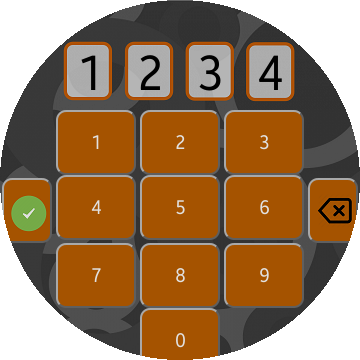
\includegraphics[width=3in]{images/login_screen.png} 
   \caption{The first version of the login screen with the small numbers.}
   \label{fig:login screen v1.0}
\end{figure}

After some testing and discussions it was decided that the feedback of the pressed numbers on the top of the screen were to small and thus some rethinking was needed to come up with a new design. An idea was to make four rotating disks that was inspired from securing a travel suitcases (see figure \ref{fig:lock}). 

\begin{figure}[H] %  figure placement: here, top, bottom, or page
   \centering
   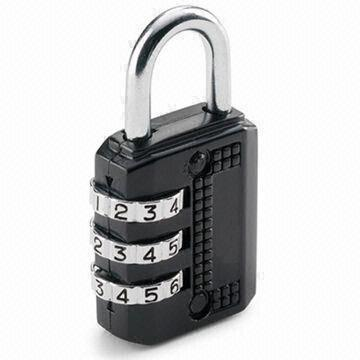
\includegraphics[width=3in]{images/lock.jpg} 
   \caption{The design of this lock was used as inspiration.}
   \label{fig:lock}
\end{figure}

The advantage is that no buttons for the numbers were needed so the numbers could be place in the middle. In the middle they can be displayed in a larger font since more space is available due to the circular shape. However, the detection of swipe events were insufficient for rotating the disks and thus the idea for rotating disks was changed to improve the functionality. The positions of the numbers stayed the same, but instead of swiping an increase and decrease button was added above and below each number (see figure \ref{fig:login screen v2.0}). 

\begin{figure}[H] %  figure placement: here, top, bottom, or page
   \centering
   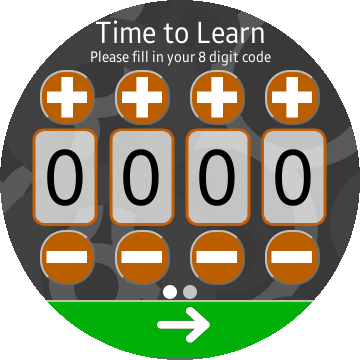
\includegraphics[width=3in]{images/login_screen_2.png} 
   \caption{The second version of the login screen with the larger numbers.}
   \label{fig:login screen v2.0}
\end{figure}

To increase the safety of a user's account it was decided to use a code of eight digits and therefore a page indicator was placed below the decrease buttons to notify the user that the user should insert 4 digits two times. On the bottom of the screen a next button is placed to go to the next page for inserting the second 4 digits of the code or to confirm that the eight digits were inserted.

\section{Main screen}

When a valid code is inserted, the main screen becomes visible. During the project, the main screen had had different layouts. All the decisions are sorted in different categories: time, words, background, buttons, information components, option lists, profile and effects.

\subsection{Time}

An important part of the app is displaying the time, since the app will be the first thing the user will see when the watch screen turns on. This importance was not clear at the beginning of the project, therefore the first design contained the time in a small black font. The size of the font was based on the hill that was displayed on the background. With the chosen font the time fitted in the hill in the middle to increase the readability (see figure \ref{fig:version1}). 

\begin{figure}[H] %  figure placement: here, top, bottom, or page
   \centering
   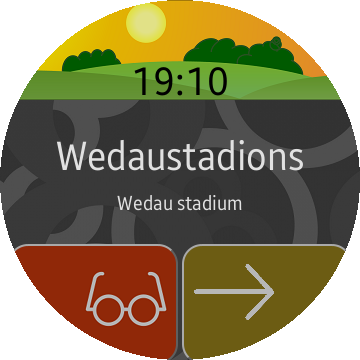
\includegraphics[width=3in]{images/version_1.png} 
   \caption{The first version of the main screen with the wrong ratio.}
   \label{fig:version1}
\end{figure}

After the first discussion it was decided that the time should be displayed on 50\% of the screen since the app would be use for checking the time and for learning words (see figure \ref{fig:version2}). The time however was not readable enough and this was solved by changing the font color to white and by changing the background (see figure \ref{fig:version3}). This new design worked well and therefore this became the final design for the time. 

\begin{figure}[H] %  figure placement: here, top, bottom, or page
   \centering
   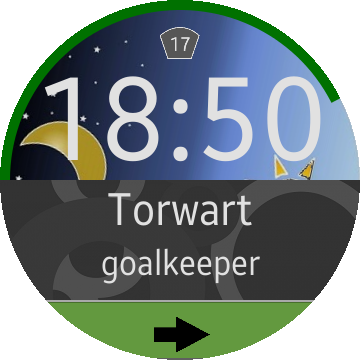
\includegraphics[width=3in]{images/version_3.png} 
   \caption{The final design of the time.}
   \label{fig:version3}
\end{figure}

\subsection{Words}

The other important part of the app is showing the wordpairs, the word and the translation, the user wants to learn. Displaying wordpairs on a small circular screen was quite challenging which resulted in different designs for the watchface (see figure \ref{fig:possible versions}). 

\begin{figure}[H] %  figure placement: here, top, bottom, or page
   \centering
   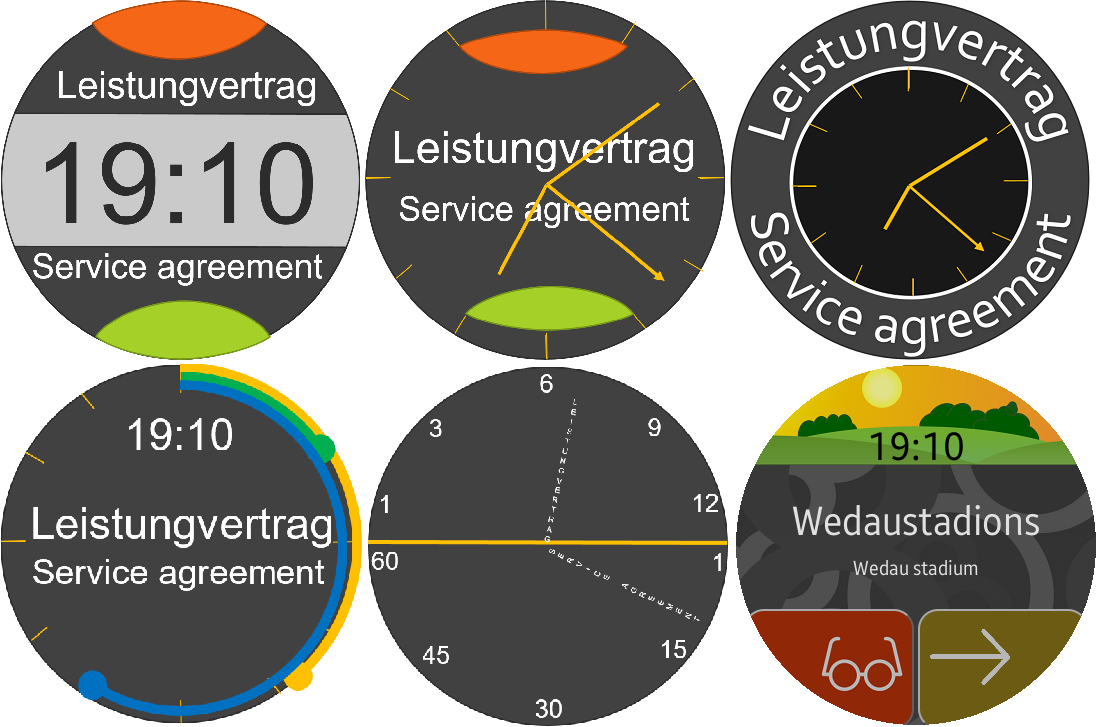
\includegraphics[width=3in]{images/all_possible_versions.png} 
   \caption{The different layouts designed for optimal usage of the circular screen.}
   \label{fig:possible versions}
\end{figure}

The sixth design was chosen as the most convincing design. In the first version the wordpairs were placed in the middle of the screen (see figure \ref{fig:version1}) with a white font. Due to the circular shape there is more space available in the middle of the screen and therefore the wordpairs can be in a larger font. The color white was chosen to have a maximum contrast with the background since the background mostly consists of dark colors. The words have a larger font than the translations to have a clear distinction between the two types and later on the smaller font was selected to make sure that there is enough space to display the translations. Since the translations are placed lower than the words, less space is available. 
When only 50\% of the screen was available for the wordpairs after the first discussion, the wordpairs were placed just below the middle where the space lost is minimal (see figure \ref{fig:version2}).  

\begin{figure}[H] %  figure placement: here, top, bottom, or page
   \centering
   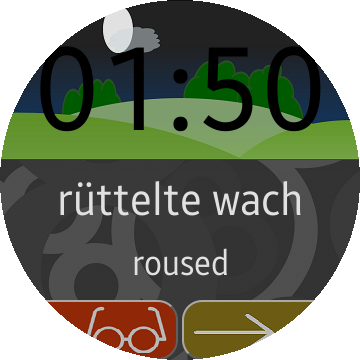
\includegraphics[width=3in]{images/version_2.png} 
   \caption{The second version of the time display uses 50\% of the screen for showing the time.}
   \label{fig:version2}
\end{figure}

\subsection{Background}

The app consists of two visual parts, one for the time and one for the wordpairs. Both parts have different backgrounds. The background for the wordpairs was selected in the beginning of the project and did not change. The background consists of different dark grayish colors. With the white colored text the user should not have any problems reading the wordpairs.

At first the idea for the background of the time was that it should support the current time. Therefore four different backgrounds were designed for the morning, afternoon, evening and night (see figure \ref{fig:first designs background}). 

\begin{figure}[H] %  figure placement: here, top, bottom, or page
   \centering
   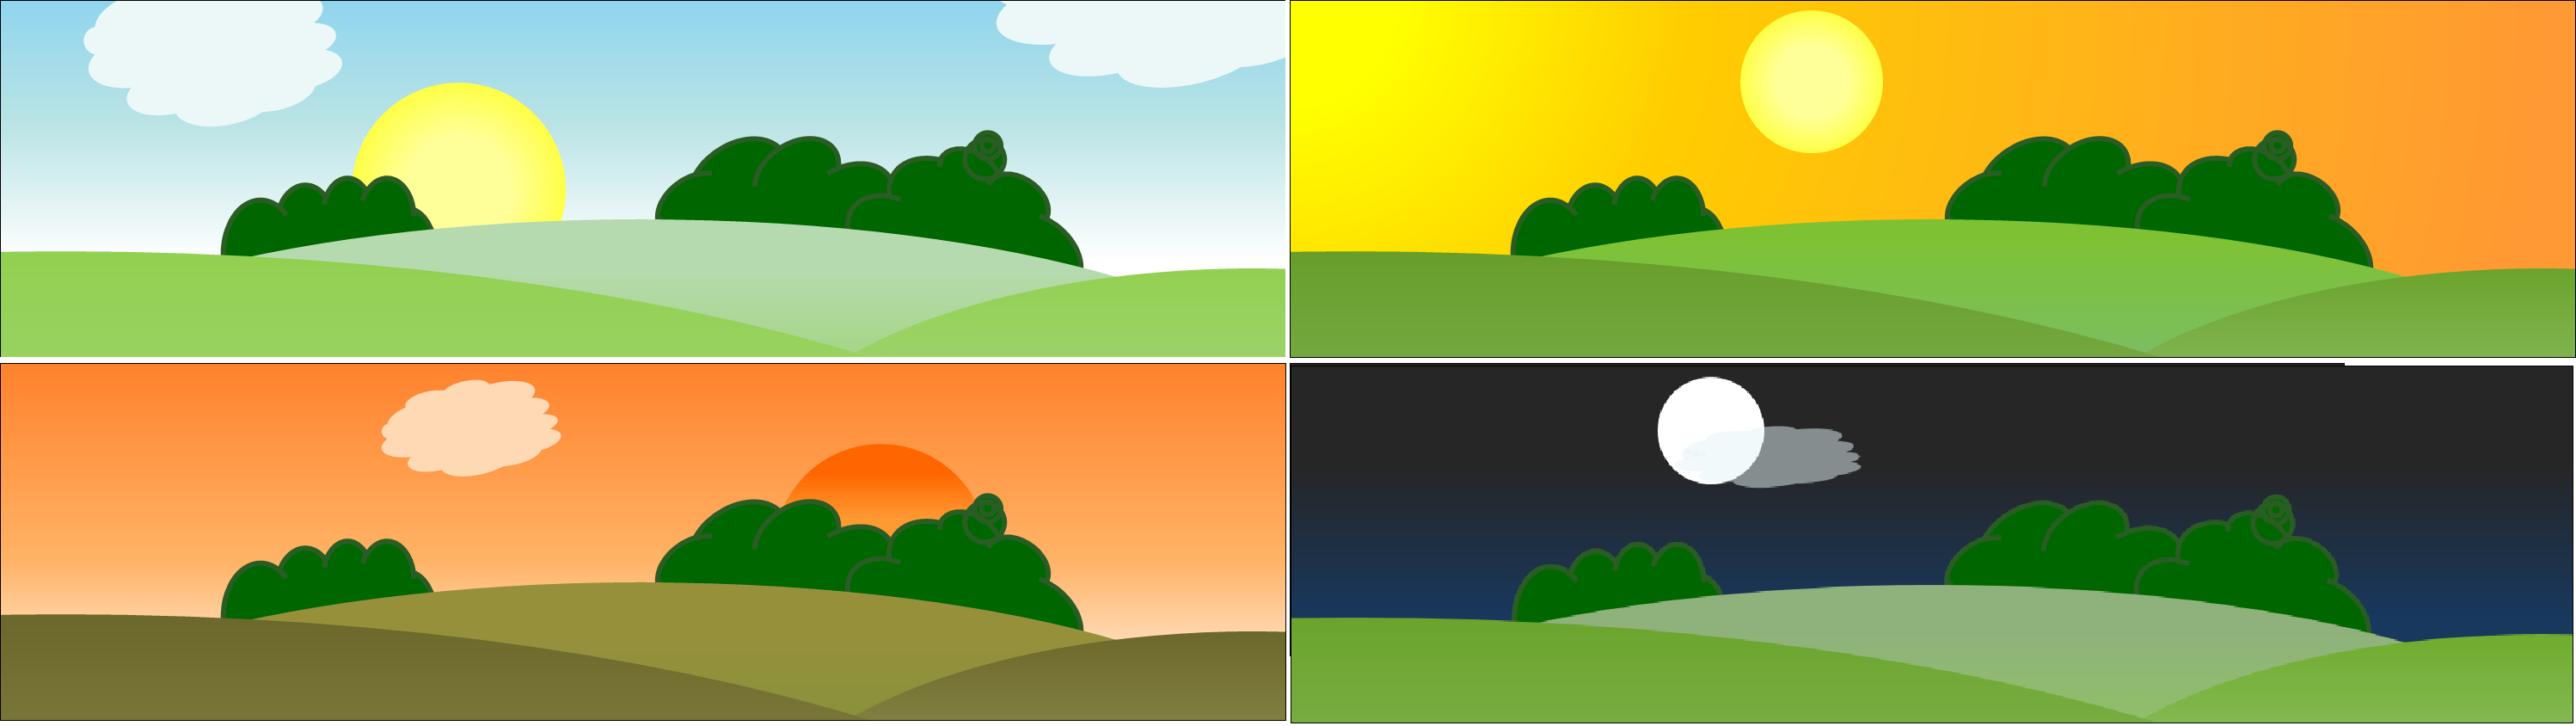
\includegraphics[width=3in]{images/first_designs_backgrounds.png} 
   \caption{The first designs for the background of the time.}
   \label{fig:first designs background}
\end{figure}

The space for the time then changed to 50\% of the screen and therefore the backgrounds were unusable because of the old dimensions of the images.
Instead of changing the images to the new dimensions this opportunity was used to think again about the background of the time. The different images for the different moments of the day had to be saved on the watch. This storage issue was solved by using one image. The new background consisted of the sun, the moon and a transition between blue and black. This background rotated around it's center which makes it possible to support the current time with the positions of the sun and the moon (see figure \ref{fig:day cycle}).

\begin{figure}[H] %  figure placement: here, top, bottom, or page
   \centering
   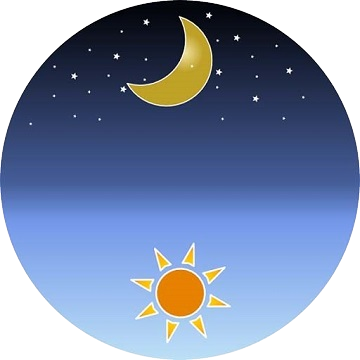
\includegraphics[width=3in]{images/day_cycle_2.png} 
   \caption{The rotating background image of the time.}
   \label{fig:day cycle}
\end{figure}

Due to the rotation a sunset and sunrise could be seen on the watch. To emphasize the sunset and sunrise a landscape was added to make, for example, the sun appear from the horizon with a sunset. The used colors for the landscape were different from the colors in the rotating background and hence a new background with the sun and moon was designed to match the landscape (see figure \ref{fig:version5}). The landscape worked well with the rotating background and therefore two other landscapes were designed from which the user can choose (see figure \ref{fig:landscapes}).

\begin{figure}[H] %  figure placement: here, top, bottom, or page
   \centering
   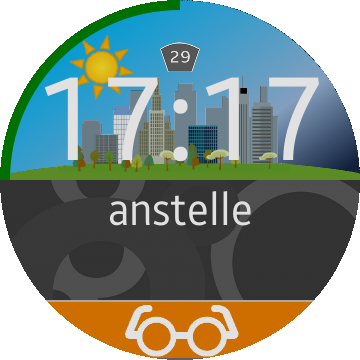
\includegraphics[width=3in]{images/version_5.png} 
   \caption{Version 5 of the main screen with a new background and a landscape.}
   \label{fig:version5}
\end{figure}

\begin{figure}[H] %  figure placement: here, top, bottom, or page
   \centering
   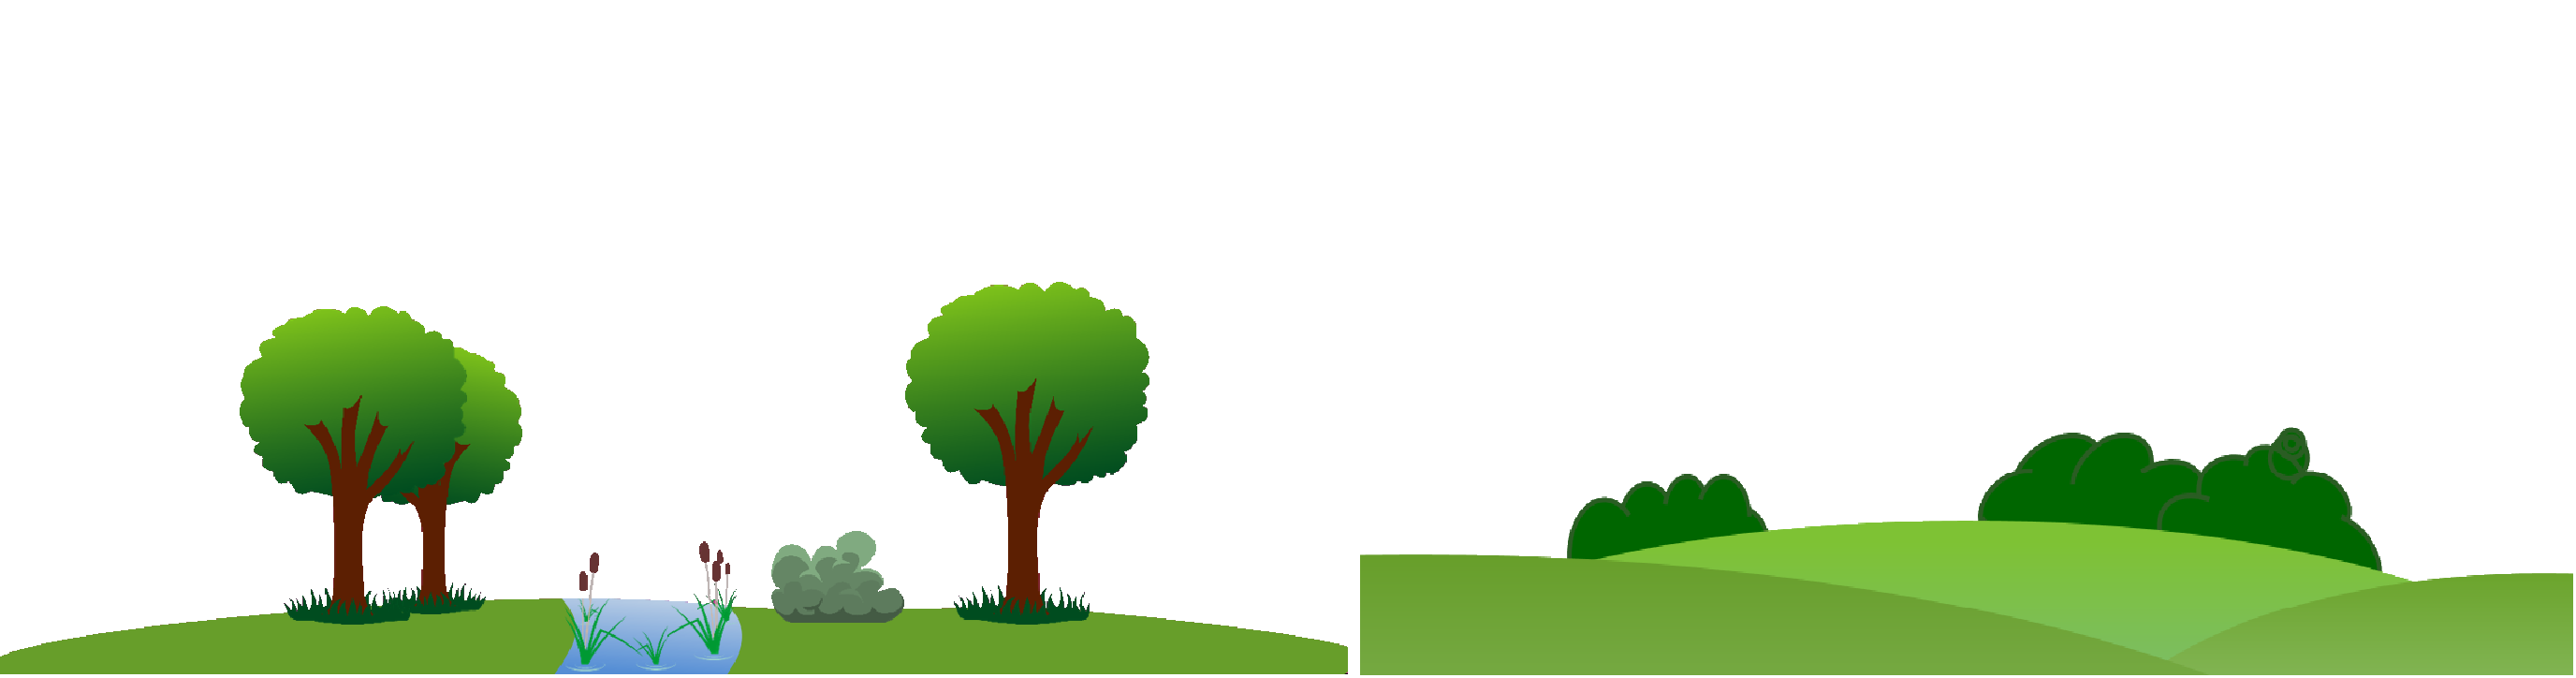
\includegraphics[width=3in]{images/designs_landscapes.png}
   \caption{The designs of the other two landscapes the user could choose from.}
   \label{fig:landscapes}
\end{figure}


\subsection{Buttons}

As mentioned before swipe detection was insufficient so it was decided that the app should only use touch events. To navigate through the app with only touch events it seemed logical to use buttons. With the time on top of the screen and the wordpairs in the middle there was unused space in the bottom for the buttons. In the first design the user should be able to 
\begin{itemize}
\item reveal the translation of the shown word, or
\item to go to the next wordpair.
\end{itemize}
This resulted in two buttons, a red one with glasses on it and one with an arrow to the right (see figure \ref{fig:version1}). Glasses were chosen for revealing because they suggest looking something up and that we found intuitive for revealing the translation.\\ 
Since the app is displayed on a small screen, the buttons should not be to small and thus almost all the available space in the bottom was used for the buttons to ensure that there was enough space for the user to press a button. Different tests showed that the buttons could be made smaller. The design of the buttons was not really pleasing and needed some rethinking. The first modification was erasing the reveal button. Instead of the button the user could touch the word to reveal the translation. The `next' button was widened so it covered the bottom of the screen (see figure \ref{fig:version3}). 
During development more options were implemented and therefore a new button was made next to the `next' button. The settings button gave access to these options (see figure \ref{fig:version4}). The curves on the buttons as can be seen in the first design were replaced with right angles to create a modern feeling.

\begin{figure}[H] %  figure placement: here, top, bottom, or page
   \centering
   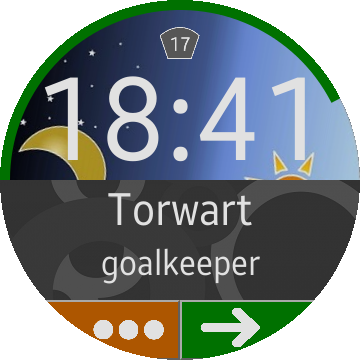
\includegraphics[width=3in]{images/version_4.png}
   \caption{Version 4 with the new `settings' button.}
   \label{fig:version4}
\end{figure}

The app was tested and more attention was paid to improve the order in which the wordpairs are shown. This process should become smarter by the use of a knowledge estimator that would estimate what the next word should be to maximize the learning process. This estimation could only be made when the server could receive feedback of every single word. It is therefore necessary that the user should give feedback after every word. The design of the app was adapted to this new idea by changing the `next' button to a `reveal' button (see figure \ref{fig:version5}). When the user pressed this button the translation appeared and the `reveal' button changed in three different buttons: a `wrong' button, a `menu' button and a `right' button (see figure \ref{fig:version5 reveal}). 

\begin{figure}[H] %  figure placement: here, top, bottom, or page
   \centering
   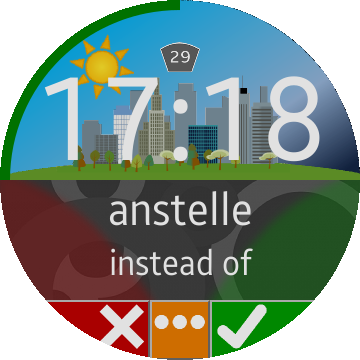
\includegraphics[width=3in]{images/version_5_reveal.png}
   \caption{The mandatory feedback page displayed after revealing a word.}
   \label{fig:version5 reveal}
\end{figure}

This new design forced the user to give feedback after every word. This feedback could be used to optimize the order of the words. The first design of the buttons were a cross and a checkmark to let the user know what to press when a word was not know or was known. Later on a book and a graduation cap were used for the same purpose but the feedback to the user would be less harsh with the new design (see figure \ref{fig:version6 reveal}).

\begin{figure}[H] %  figure placement: here, top, bottom, or page
   \centering
   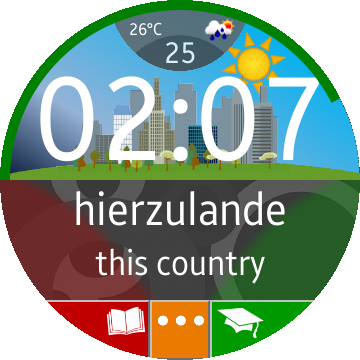
\includegraphics[width=3in]{images/version_6_reveal.png} 
   \caption{The mandatory feedback page with the redesigned buttons}
   \label{fig:version6 reveal}
\end{figure}

\subsection{Information components}

Besides the time the app also shows the date. The date was added later when the design of the time was completed. In the first design the date had his own small icon on top of the screen (see figure \ref{fig:version3}). This icon was partly covered by a Tizen icon for the swipe down menu. Therefore the icon for the date was moved downwards near the time (see figure \ref{fig:version5}).
During a discussion it was mentioned that it would be nice to be able to see the temperature and the weather type on the watchface. After some research a free API\footnote{http://openweathermap.org/}was found that could provide the app with this information. In the beginning of the implementation the temperature was placed to the left of the date and the weather type was placed to the right of the date. This was barely readable and it did not fit in the realized design hence a new icon was designed that contained the date, temperature, weather type and an open area in the middle for the Tizen icon for the swipe down menu (see figure \ref{fig:version6}).

\begin{figure}[H] %  figure placement: here, top, bottom, or page
   \centering
   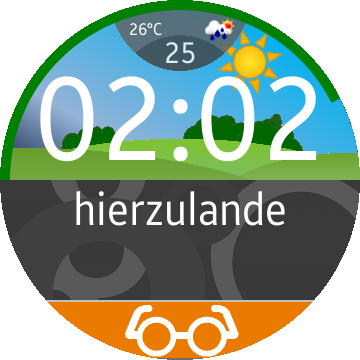
\includegraphics[width=3in]{images/version_6.png} 
   \caption{Version 6, the final design}
   \label{fig:version6}
\end{figure}

\subsection{Option lists}

The app has access to two different option lists: 
\begin{itemize}
	\item the settings which can be reached by double tapping on the time, and 
	\item the menu that can be reached by tapping in the middle of the translation. 
\end{itemize}
The app started with one option list. When the app was able to show the words with the translation, the user should have an option to tell the app that a word had a wrong translation or that a word was learned and thus in both cases it should not reappear again. Due to the small screen it was not convenient to add more buttons for each of these options to the watchface and therefore we decided to make a menu with these extra options. 

Besides these options the user should be able to reverse the order in which the wordpairs were asked (when the words were displayed from German to English, the words would be displayed from English to German after the button was pressed), to insert the number of words that the user wanted to learn and to log out of the app. All these options were reachable for the user by a 'menu' button in the bottom. The 'next' button was replaced by two buttons, the 'menu' and the 'next' button (see figure \ref{fig:version4 menu}). 

\begin{figure}[H] %  figure placement: here, top, bottom, or page
   \centering
   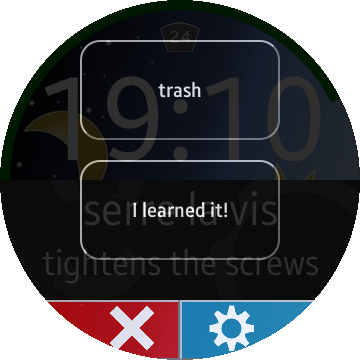
\includegraphics[width=3in]{images/version_4_menu_1.png}
   \caption{The design of the menu in version 4.}
   \label{fig:version4 menu}
\end{figure}

In the bottom the user could close the menu or open the settings. By pressing the `settings' button the user would open the settings page with the buttons for reverse, number of words and log out (see figure \ref{fig:version4 settings}).

\begin{figure}[H] %  figure placement: here, top, bottom, or page
   \centering
   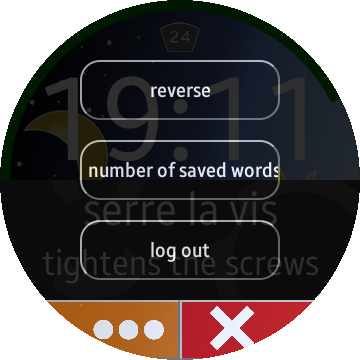
\includegraphics[width=3in]{images/version_4_settings_1.png}
   \caption{The design of the settings in version 4.}
   \label{fig:version4 settings}
\end{figure}

After some discussions the overall opinion was that the 'menu' button should not be this large on the watchface since the menu would give complementary options which were not part of the main function of the app. Therefore the button should not cover half of the bottom and a solution was to split the menu and the settings to two different pages that the user could reach independently. The user could reach the menu by tapping in the middle of the translation (see figure \ref{fig:version5 reveal}) and the settings could be reach by double tapping on the time since this space was hardly used. The double tap was necessary because tapping the time was already assigned to changing the background.
The menu and the settings both had a black transparent background for a long time. This was inspired from the transparent and blurred swipe down menu from a well-known OS. Unfortunately the blur effect was not a success, but the transparency remained.

During testing the text in the buttons were hard to read and the buttons of the main page were visible through the buttons on the bottom. Therefore it was decided that the menu and the settings page should have a background. For the background the same image was used as the background of the wordpairs to preserver the unity of the design.
Many translations depend on the context of a word. Hence the user should be able to see the context of the word and this option was added to the menu page (see figure \ref{fig:version6 menu}).

\begin{figure}[H] %  figure placement: here, top, bottom, or page
   \centering
   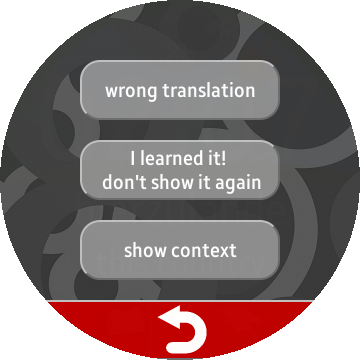
\includegraphics[width=3in]{images/version_6_menu.png} 
   \caption{The new design of the menu in version 6.}
   \label{fig:version6 menu}
\end{figure}

Later the idea was abandoned of letting the user choose how many words the user wants to learn. The 'profile' button was the latest addition to the settings page (see figure \ref{fig:version6 settings}).

\begin{figure}[H] %  figure placement: here, top, bottom, or page
   \centering
   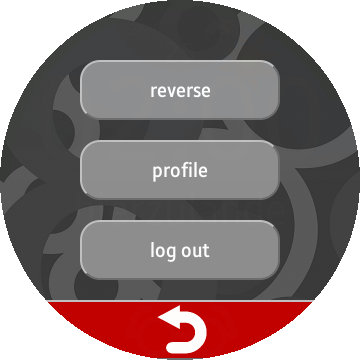
\includegraphics[width=3in]{images/version_6_settings.png} 
   \caption{The new design of the settings in version 6.}
   \label{fig:version6 settings}
\end{figure}

\subsection{Profile}

The app has a profile page where the user can see the four medals that can be earned by using the app (see figure \ref{fig:version6 profile}). The four categories are: words learned, total time, longest session and longest streak. 

\begin{figure}[H] %  figure placement: here, top, bottom, or page
   \centering
   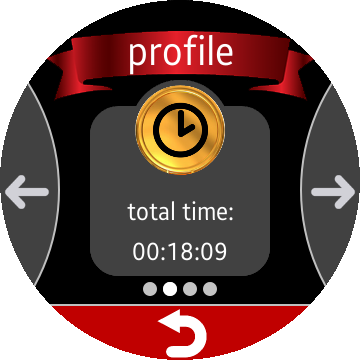
\includegraphics[width=3in]{images/version_6_profile.png} 
   \caption{The profile page in which the user can find the latest earned achievements.}
   \label{fig:version6 profile}
\end{figure}

The idea was that when users can earn medals, they would be more willing to use the app. 
When the user presses the 'I learned it' button, the number of 'words learned' will increase and after 10 new learned words, a popup will appear with a motivating message to continue. 

The total time the user used the app is also registered. When this time is the same as one of the pre-determined minutes a popup appears (see figure version 6 popup.png).
With longest session the time is measured that the user uses the app  continuously and with the longest streak the number of days is registered in which the app is used daily. One day of not using the app resets the longest streak.

\begin{figure}[H] %  figure placement: here, top, bottom, or page
   \centering
   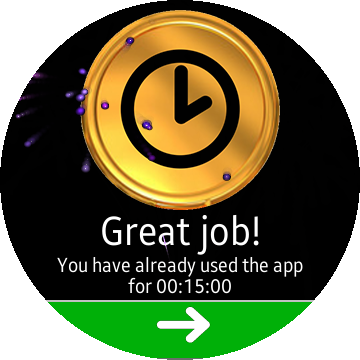
\includegraphics[width=3in]{images/version_6_popup.png} 
   \caption{The design of the popup screen when the user improved an achievement.}
   \label{fig:version6 popup}
\end{figure}

\subsection{Effects}

To improve the experience of the app some effects were added: to give feedback after a button was pressed, to give information (why an option was not available or why a medal was earned) or to beautify a popup.

Because of the small screen the user could think the wrong button was pressed and therefore the user should get feedback about which button was pressed. The most important buttons in the app are the buttons used for indicating whether a word was known or not. When one of these buttons is pressed a green or red image appears depending on if right or wrong is pressed. This image stays on the display for a few milliseconds before it fades out.

In the app several popups are added to give the user feedback when an option is not available. The design of the popup is based on the first design of the option lists. The popup has a black transparent background with white text on it. The popup could appear when: there is no connection with the internet, when a wrong code is inserted, when the user has too few words, when there are too few words left on the watch or when a user earned a new medal.
The popup that appears when a new medal is earned is beatified by a particle animation representing fireworks.


\chapter {The Implementation}
In this part the implementation choices are described. In this project writing the code was one of the biggest challenges. The code has been changed a lot during the process. One of the reasons was to increase readability, but also because of design changes and new features which had to be implemented. The code is written in JavaScript in combination with HTML 5, the main web technologies at the moment. The code is build with a framework called require.js, this makes it possible to have multiple files (modules) in javascript, in order to increase readability and structure. In the following sections, we will zoom in some interesting and important decisions and choices related to the implementation.

\section{Flash card algorithm}
For presenting the words we used an algorithm which will make sure users will learn faster. The algorithm is based on the flashcard method (see fig. \ref{fig:flashcard simulation}). The algorithm works in such a way that the user is able to give feedback in the form of `wrong' and `right'. The words which are marked as `wrong' will be faster repeated than words which were marked `right'. As explained in the design the user must indicate whether he had the answer wrong or right in his head. If the user had it wrong the word will be repeated after five more words, when the user had it right the timing when the word will be repeated depends on the number of times the user had it correct. The word will be $timesCorrect * 5$ positions moved in case the user had it right in his head. 

\begin{figure}[H] %  figure placement: here, top, bottom, or page
   \centering
   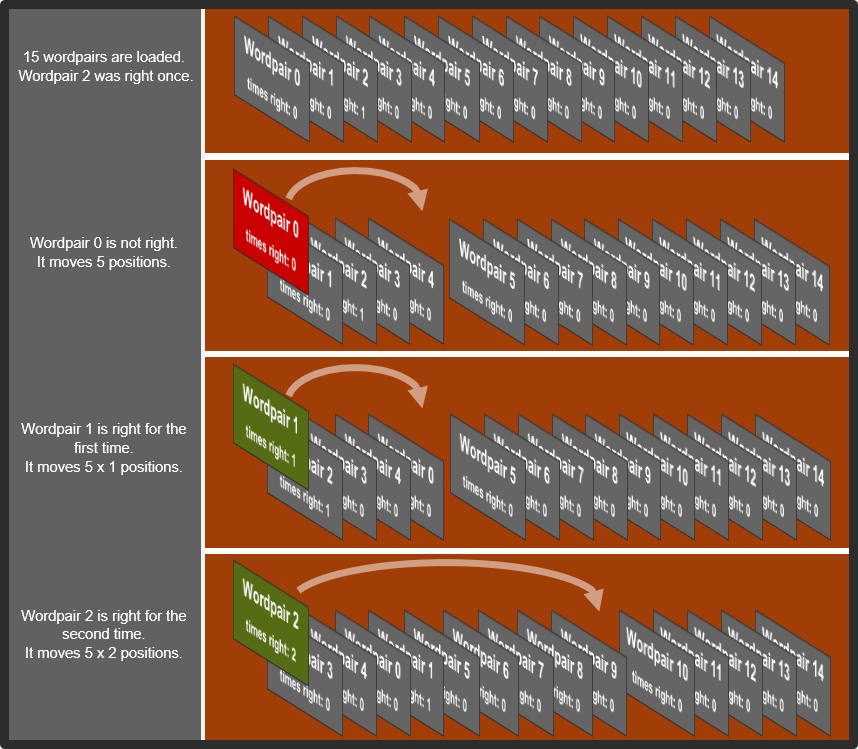
\includegraphics[width=\linewidth]{images/flashcard_method.png} 
   \caption{An example Flashcard simulation}
   \label{fig:flashcard simulation}
\end{figure}

Every time the user taps wrong or right the function $updateWordPair$ is called (see listing \ref{flashcard}). If the user is right the number of times correct will be increased. After that the current word will be moved in the array. This happens by first adding the word some positions further and then deleting the current word (i.e., deleting element zero in the array). If the user was wrong the current progression will be reset (i.e., timesCorrect becomes zero again), and the word will be moved five positions to the right (see figure \ref{fig:flashcard simulation}). This means the word will be repeated reasonably fast. 

Because the first element of the array is always shown on the screen, the next word will be drawn on the screen, since the previous first element is deleted. In $userData.js$ everything related to the user is implemented, so this is the place where words can be found. A wordPair is characterized with the following attributes: word, translation, id, context and number of times correct. Getting the word pairs from the server is explained in the next section.

\lstinputlisting[label=flashcard, language=JavaScript, firstline=49, lastline=59, caption=flashcard implemenation in userData.js]{source_code/userData.js}

\section{Getting new words from the server}
The module \module{session.js} declares function $getWords$ which fetches words from the server. The module \module{session.js} is loaded in the module \module{main.js}, there the function $session.create$ is called. This function takes the login code, which is provided by the \module{login.js} module (i.e., entered by the user or loaded from the userData). This module is also loaded in \module{main.js}. The login code is required to be submitted with every request to the server. The code is unique for every user. The login code can be found in the account when logged in the browser. The code contains eight digits. When a session is created, the first thing to look at are there currently any words on the watch. If there are any words on the watch we can set the status to `success', in case there are no words on the watch yet: the watch has to communicate with the server and get the words with the endpoint `bookmarks\_to\_study'. This endpoint will return the words which are currently the most important to study for that particular user. In the implementation we made the choice to get fifty words in case the user has no internet connection for longer periods of time. The session can return different states: if the words are successfully fetched from the server the state will be `success' as described earlier, if the code is invalid the state will be `wrong session number', in case of no internet connection the state will be `no connection'. There is one exception, but this will not happen very often this is when there are too few words in the account of the user. One of these states will be returned to the main module and the main module will give this state through to the login module, in the login the user can then be informed by a popup that will inform the user about a specific situation. If the state was `success' the user will get in the main screen where the words are presented. The login module is not the only place where the watch tries to get new words, it also happens when the user is already logged in and a screen on event occurred (i.e., user makes arm twist to look at time). The new words will then be added to the current wordlist on a screen off event (i.e., user makes again a arm twist to indicate he is not looking anymore), adding words at this point is to prevent any conflicts: adding words to a list which the user is currently doing stuff with. New words will only be added if the list is smaller than fifty words. The list can become smaller if the user has marked a couple of words as `learned it' or as `wrong translation'. When writing the code the initial preference was to get words and add them at the same time on a screen off event, since the user won't be using the application at that moment and it would really feel as everything happens in the background. Unfortunately this didn't work the watch gets in a sort of sleep modus and won't be able to communicate with server anymore. The GET request wasn't executed so it was impossible to do this on a screen off event. When the watch tries to get new words from the server, this happens asynchronously to prevent the watch from getting slow. Implementing this asynchronously was huge in the end, because the user is able to get a lot of words in his account (e.g., some user had already 10000 words) the endpoint will be really slow, since the list of words is not already sorted on importance on the server server side. In the first implementation when it was implemented synchronously, therefore the user could have some delay before being able to interact with the watch. It was first implemented in this way to prevent conflicts, user cannot do something with a list while words are being added. This is now solved by getting the new wordPairs on a screen on (see listing \ref{new wordPairs}) and add them later on a screen off (see listing \ref{add new words}).

\lstinputlisting[label=new wordPairs, language=JavaScript, firstline=48, lastline=62, caption=getting new wordPairs in session.js]{source_code/session.js}

\lstinputlisting[label=add new words, language=JavaScript, firstline=32, lastline=35, caption=adding new words to wordPair in userData.js]{source_code/userData.js}

\section{Usage Tracking}

\subsection{Events}
Events are implemented to give the knowledge estimator information which can be used to analyze the knowledge of the user. The knowledge estimator is on the server side implemented. This means we had to decide at what point we should send the events. Because the knowledge estimator decided what the next word is going to be for the user, the events should be send when the user taps wrong or right. This is the moment the user will be presented with a new word. The knowledge estimator can receive the following events: reveal, right, wrong, wrong translation, I learned it, showContext, screenOn and screenOff. 

\subsection{Clicktracking}
The clicktracker is designed for research purposes. Its purpose is to track where the user clicks/taps, so the coordinates are saved. Not only the click position is saved, also the click type (e.g., user taps on reveal). For some functions this can be really interesting like the right button; the user can tap on the button itself or on the green space above the button. Both actions result in the same thing. In the future we could change the design based on these results to give the user a better experience. To conclude the clicktracker is not implemented as an extra function for the user, it is purely for research purposes.

\section{Changing the watchface and sending and saving}
Sending and saving the clicks and events was a big challenge in this project. This is the result of the user being able to change the watch face at every moment, which will result in losing data. Because the user is able to go to a different watch face at any moment clicks and events should be saved to the storage of the watch immediately. We do this by saving it to the local storage. This is implemented in the same way as saving to the local storage in a web browser. A click and event are immediately pushed to the storage after they occurred. The clicks in the storage are sent on a screen-on event asynchronously, so it won't influence the speed of the application and it happens in the background. When the clicks are successfully sent to the server, the server will return `OK', if the watch then receives this message the clicks in the storage can be freed, they are now at the server. The events in the storage are sent on `right' and `wrong' as previously explained to inform the knowledge estimator. Just as with the clicks the events are deleted from the storage if they successfully have been arrived on the server side. Losing data with changing the watch face not only happens with clicks and events, it also happens when the user reverses the way the words are asked (e.g., English - Dutch to Dutch - English) and with changing the background. The login code is being saved the first time and used for automatic login after a watch face change. 

\section{Drawing the user interface}
The user interface is drawn every second on the screen, this happens in gui.js in the draw function which is public (shown in listing \ref{draw function}). The main module has an function which calls this function in GUI every second (shown in listing \ref{main}). The screen is thus updated every second. Time and profile are also being refreshed in the draw function, in the future it would be nice to have these in a different function to make sure the function only draws. 

\lstinputlisting[label=draw function,language=JavaScript, firstline=153, lastline=163, caption=draw function in gui.js]{source_code/gui.js}

\lstinputlisting[label=main, language=JavaScript, firstline=11, lastline=14, caption= updateScreenEverySecond function in main.js]{source_code/main.js}

\chapter{Usage Study}
After the implementation the app was ready to enter the test phase. The results of the test period should give answers to the following two questions: is the app used during short intervals (this would indicate that the users used the app for micro learning) and is the app designed properly (e.g., are all the options found during the test period).

The test period consisted of four parts:
\begin{enumerate}
\item All participant started with making an account on Zeeguu and used Zeeguu Reader for reading. During this usage, the platform saved words they did not understand.
\item The participant received the smartwatch with the app as a watchface and basic instructions about how to use the app.
\item The participant used the app for four days in a row.
\item After four days the participants handed in the smartwatch and they filled in a questionnaire about the test period and how they experienced the app.
\end{enumerate}

During the test period the smartwatch kept track of the usage by using telemetry. All the buttons and touch areas for the existing options had different events attached to them so when a button or area was pressed, an event would be sent to the server. The events and their definitions are shown in table \ref{events}. 

\begin{table}[H]
\centering
\caption{Events}
\label{events}
\begin{tabular}{| l | p{10cm} |} 
\hline
\textbf{Type} & \textbf{Definition} \\ \hline 
screenOn & The screen lightens up. \\ \hline
reveal & The user wants to see the translation and presses the `reveal' button or area. \\ \hline
right & The user knows the translation and presses the `right' button or area. \\ \hline
wrong & The user does not know the translation and presses the `wrong' or area. \\ \hline
wrongTranslation & The user thinks the translation is incorrect and presses the `wrong translation' button in them menu. \\ \hline
learnedIt & The user thinks the word is learned and presses the `I learned it' button in the menu. \\ \hline
showContext & The user wants to see the context of the word and presses the `show context' button in the menu. \\ \hline
reverse & The user wants to learn the other way around and presses the `reverse' button in settings. \\ \hline
screenOff & The screen turns off (automatically, after a timeout or arm twist). \\ \hline
\end{tabular}
\end{table}

\section{Usage results}
After all the participants finished their test period all the events per user were collected from the server and analyzed. For answering the research questions and for giving a clear overview about how the app was used during the test period, the following diagrams were made per user: 
\begin{itemize}
\item A pie chart diagram presenting the overall usage of the smartwatch in seconds
\item A pie chart diagram about the duration of the learning sessions on the app in seconds
\item A bar chart about the number of times a user pressed `right' and `wrong'
\item A table with the median reaction time between a `reveal' and a `right' or `wrong' and the time the app was used
\end{itemize}


\subsection{Pie chart diagram presenting overall usage in seconds.}
This diagram (see fig. \ref{fig:general usage 1 2} and \ref{fig:general usage 3 4}) was created by collecting all the time intervals between a `screenOn' and a `screenOff' event. This data was then sorted into five different intervals:
\begin{itemize}
\item time $\leq$ 2
\item 2 $<$ time $\leq$ 5
\item 5 $<$ time $\leq$ 15
\item 15 $<$ time $\leq$ 60
\item time $>$ 60
\end{itemize}
The first interval was chosen, assuming that checking the time or other arm movements would not take more than two seconds. When the duration is longer than two seconds the user probably does more than only checking the time. 
The user could check the time, but because a word is shown too, the user might reveal that word by pressing `reveal' and then the user might also give feedback by pressing `right' or `wrong'. These actions for one word would take not more than five seconds. Summarized, these could be learning sessions that were not intended to be a learning session. Then comes the intended learning sessions but for a really short time and the sessions that took a bit longer. As mentioned before the learning app will probably only be used for short sessions and thus sessions longer that one minute will probably hardly occur.
\textbf{A pie chart diagram about the duration of the learning sessions on the app in seconds (see fig. \ref{fig:learning sessions 1 2} and \ref{fig:learning sessions 3 4}.).} 
The durations of the learning sessions were found by using an algorithm (see listing \ref{script}). This algorithm first sorted out all the `screenOn' events that were immediately followed by a `screenOff' event. A user that used the app for learning and not for checking the time would use at least one option the app provides for learning new words before the screen would turn off. Therefore the combinations of a `screenOn' and `screenOff' events were seen as not learning sessions and these pairs were erased from the list of events\footnote{There is possibly some noise here as a user might have left the word and the translation on the screen and see them displayed nevertheless}. 
In the remaining events the time was measured between a `screenOn' and a `screenOff' event and afterwards the data was sorted into four intervals: 
\begin{itemize}
\item time $\leq$ 5
\item 5 $<$ time $\leq$ 15
\item15 $<$ time $\leq$ 60
\item time $>$ 60
\end{itemize}
The app will presumably be used for micro learning. Therefore the number of sessions will probably decrease exponentially when the duration increases. This is the reason why the length of the intervals increases faster than a linear growth.
\textbf{A bar chart about the number of times a user pressed `right' and `wrong' (see fig. \ref{fig:right wrong 1 2} and \ref{fig:right wrong 3 4}).} 
For each day the app was used the number of `right' and `wrong' events were counted and plotted in a bar chart. 
\textbf{A table with the median reaction time between a `reveal' and a `right' or `wrong' and the time the app was used (see tables \ref{table time 1}, \ref{table time 2}, \ref{table time 3} and \ref{table time 4}).} The reaction time is the time it took the user to press `right' or `wrong' after `reveal' was pressed. The average was calculated for each single day and for the whole period of four days. Besides the average time the total time is mentioned too. This indicates for how long the user used the app during the four days of testing.

\begin{figure}[H]%
    \centering
    \subfloat[User 1]{{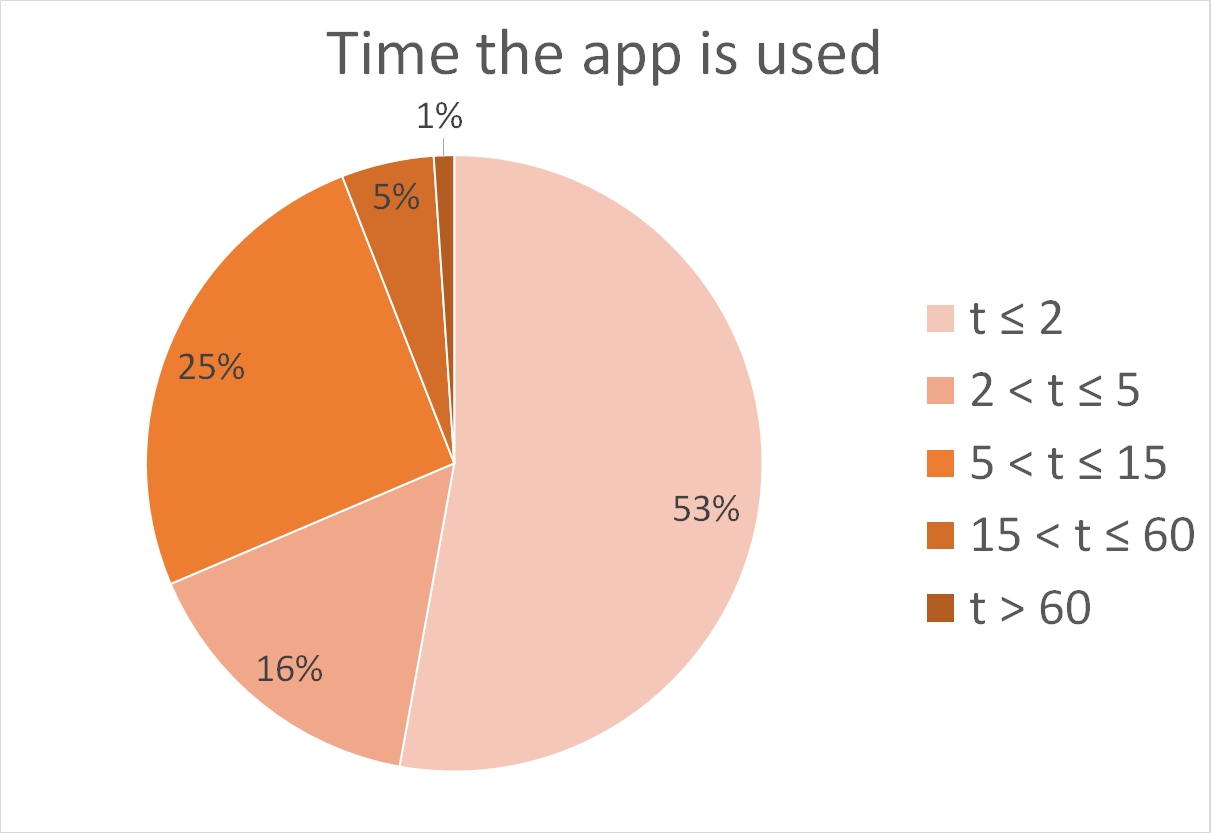
\includegraphics[width=2.6in]{usage_results/1_usage.png} }}%
    \qquad
    \subfloat[User 2]{{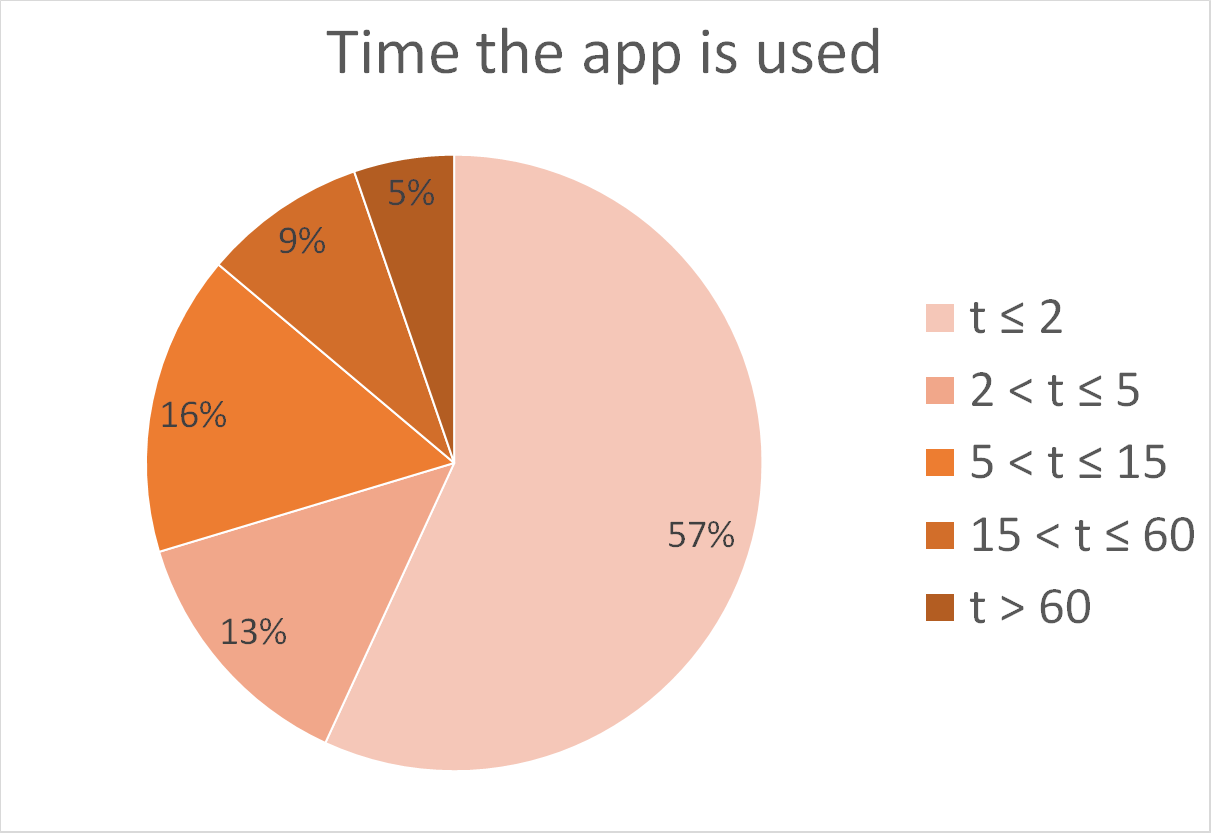
\includegraphics[width=2.6in]{usage_results/2_usage.png} }}%
    \caption{General usage users 1 and 2}%
    \label{fig:general usage 1 2}%
\end{figure}

\begin{figure}[H]%
    \centering
    \subfloat[User 3]{{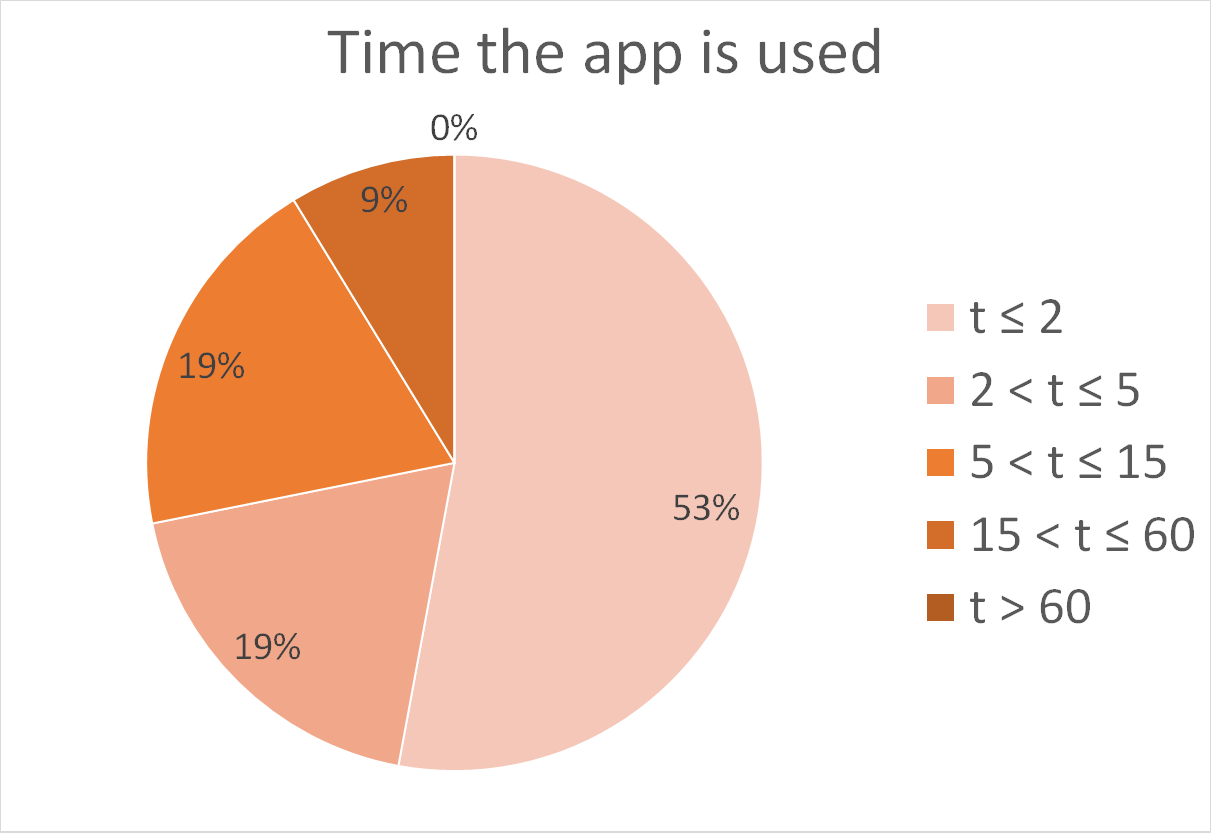
\includegraphics[width=2.6in]{usage_results/3_usage.png} }}%
    \qquad
    \subfloat[User 4]{{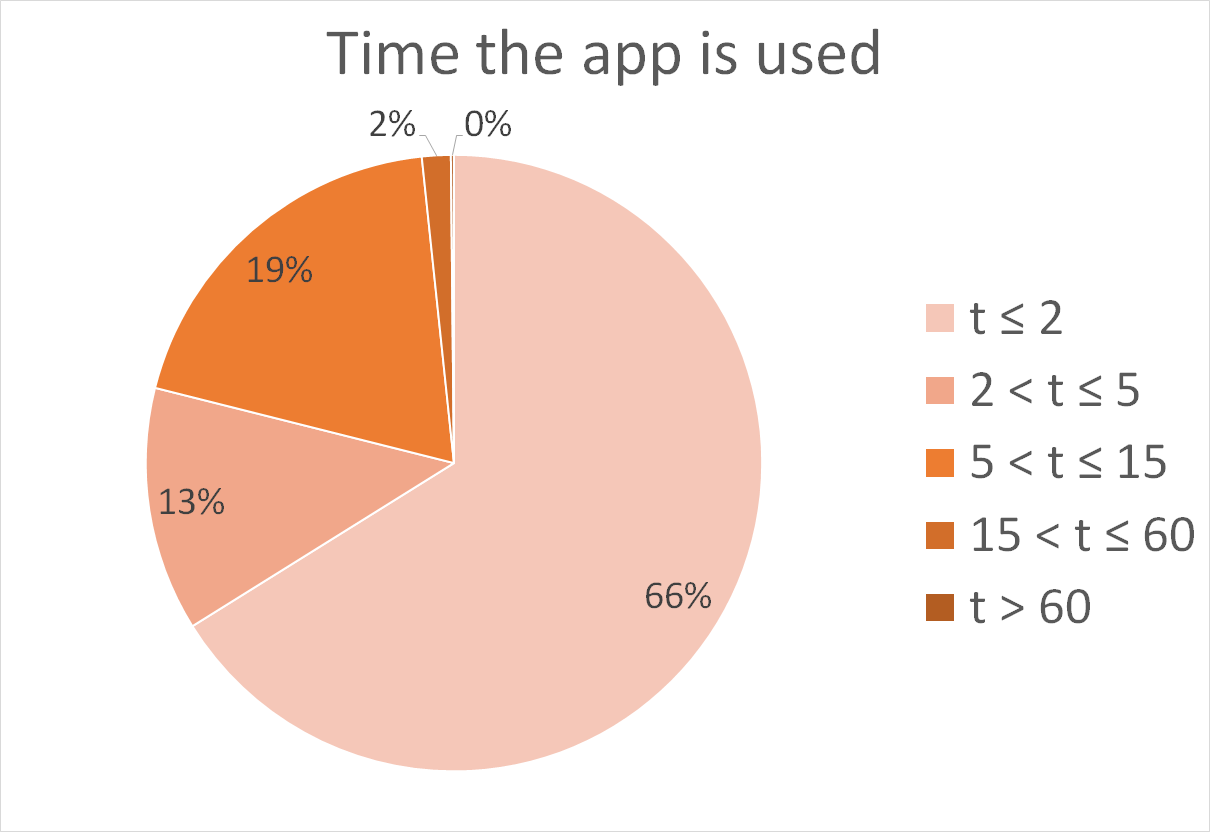
\includegraphics[width=2.6in]{usage_results/4_usage.png} }}%
    \caption{General usage users 3 and 4}%
    \label{fig:general usage 3 4}%
\end{figure}

\begin{figure}[H]%
    \centering
    \subfloat[User 1]{{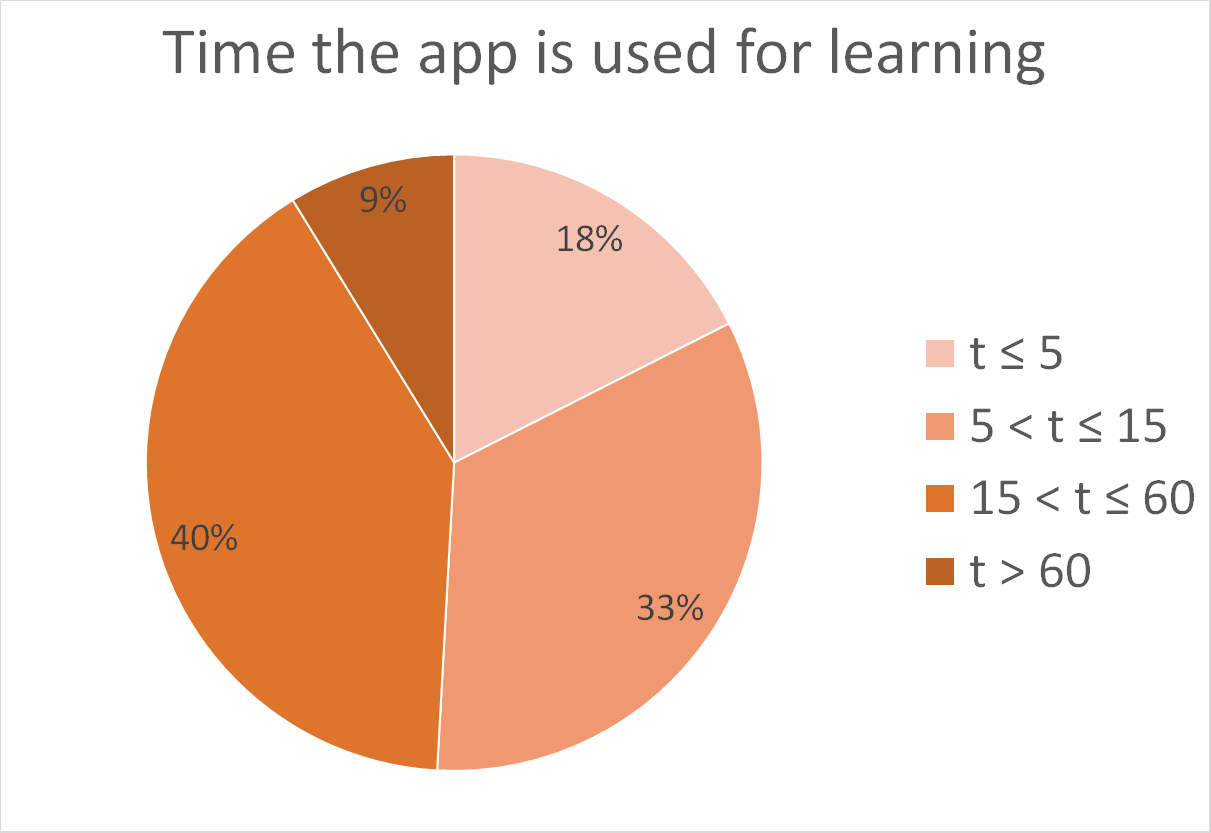
\includegraphics[width=2.6in]{usage_results/1_usage_learning.png} }}%
    \qquad
    \subfloat[User 2]{{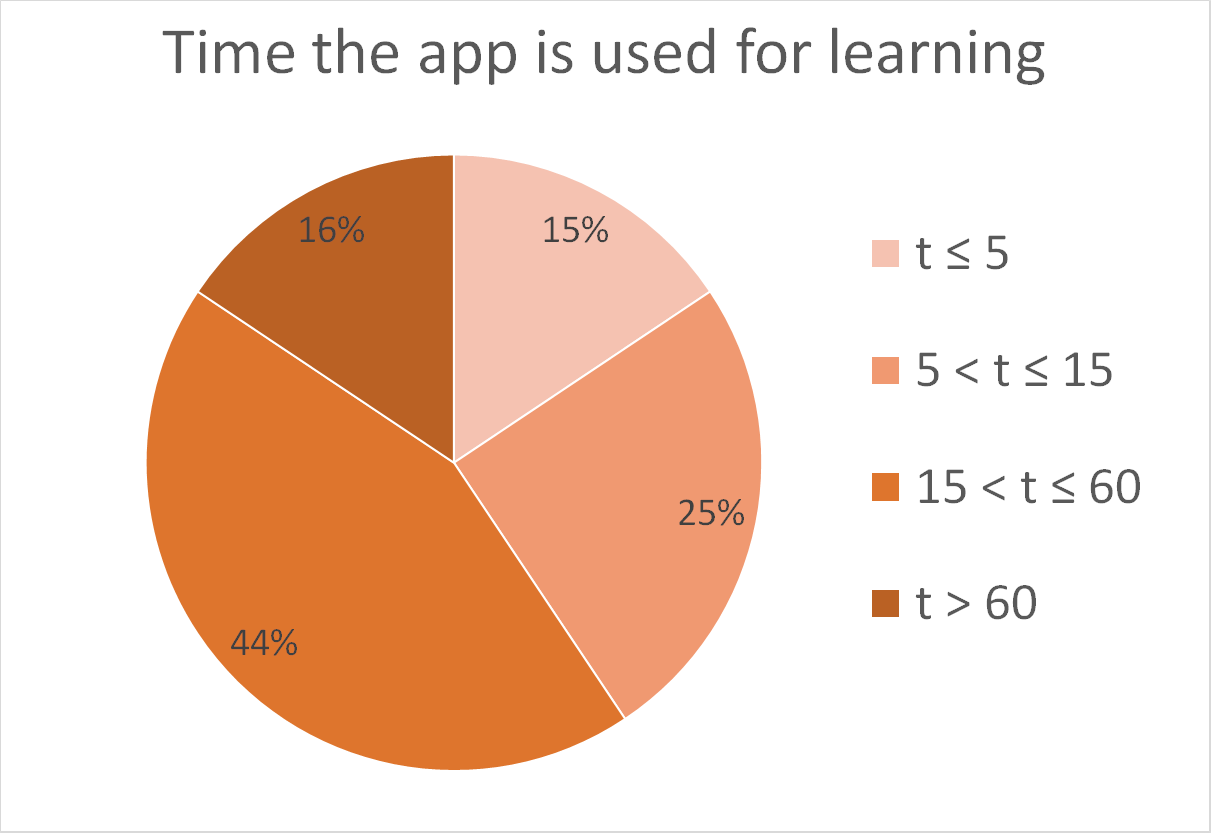
\includegraphics[width=2.6in]{usage_results/2_usage_learning.png} }}%
    \caption{Learning sessions time users 1 and 2}%
    \label{fig:learning sessions 1 2}%
\end{figure}

\begin{figure}[H]%
    \centering
    \subfloat[User 3]{{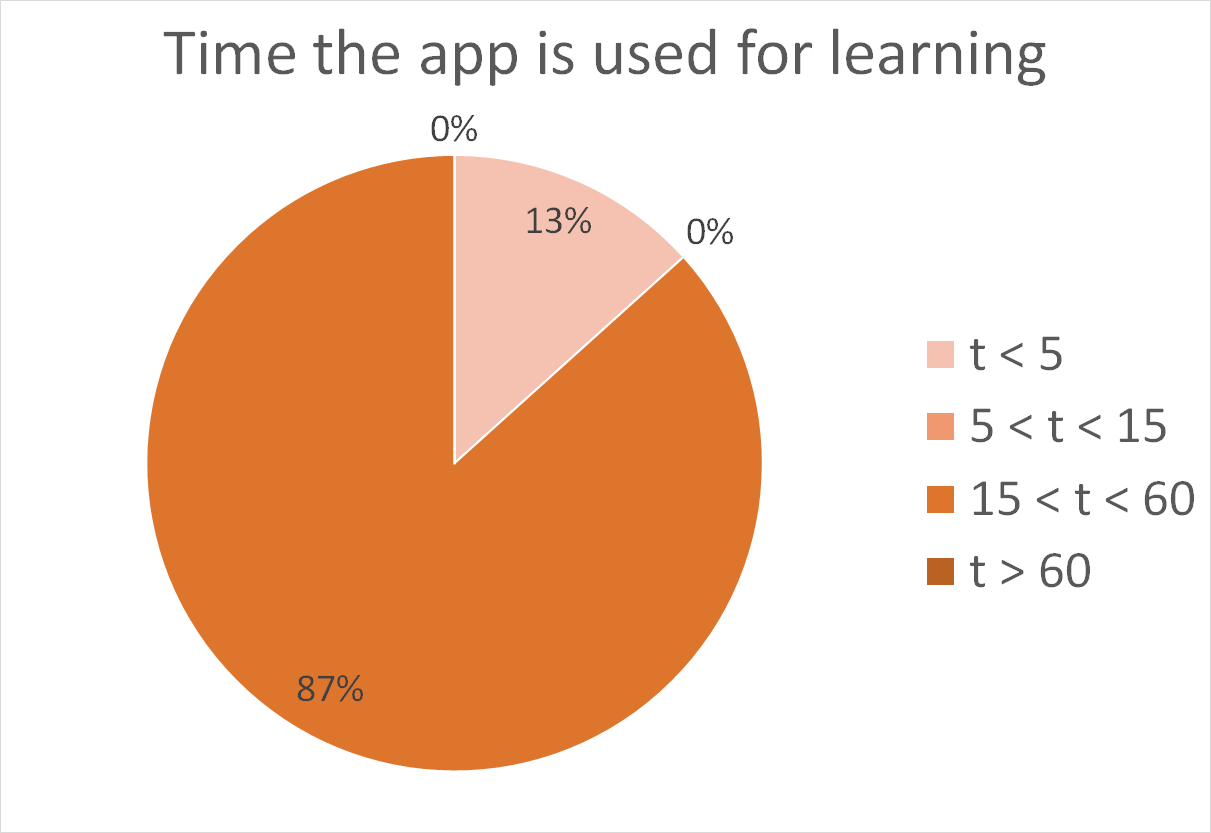
\includegraphics[width=2.6in]{usage_results/3_usage_learning.png} }}%
    \qquad
    \subfloat[User 4]{{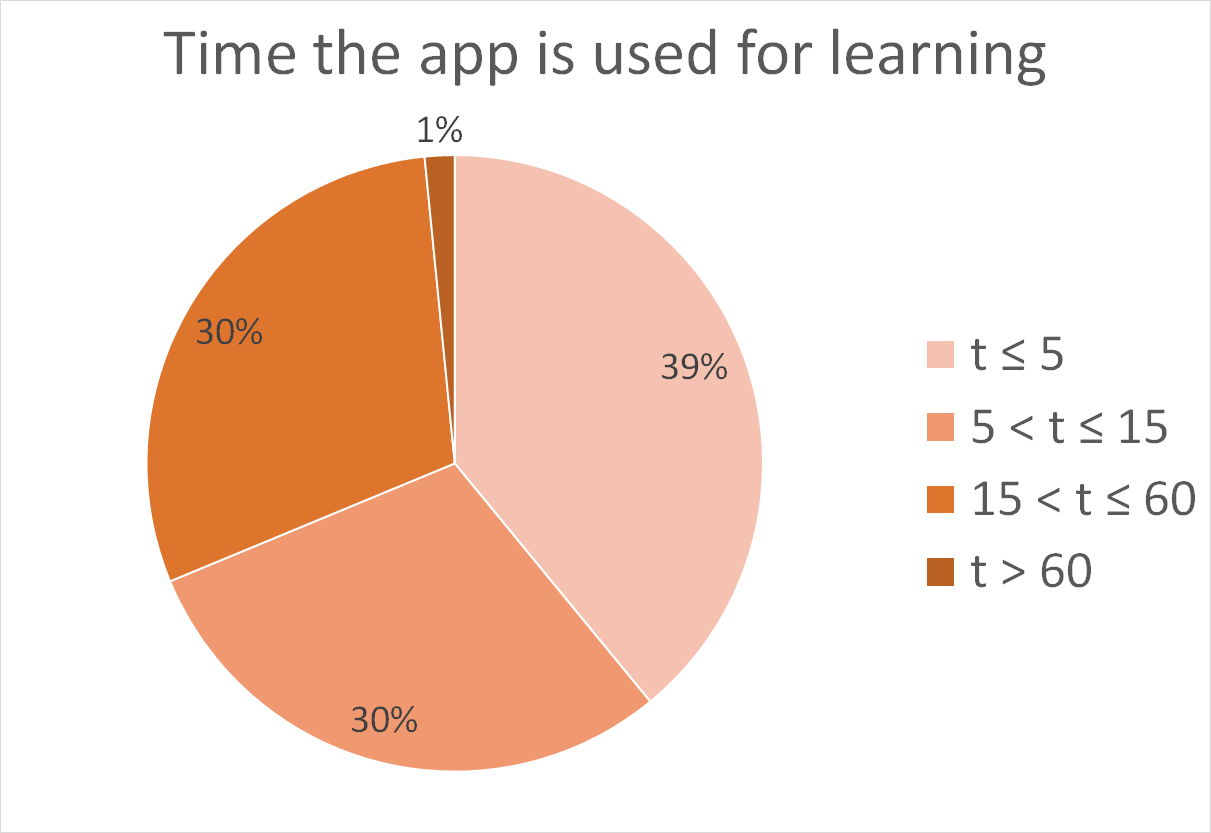
\includegraphics[width=2.6in]{usage_results/4_usage_learning.png} }}%
    \caption{Learning sessions time users 3 and 4}%
    \label{fig:learning sessions 3 4}%
\end{figure}

\begin{figure}[H]%
    \centering
    \subfloat[User 1]{{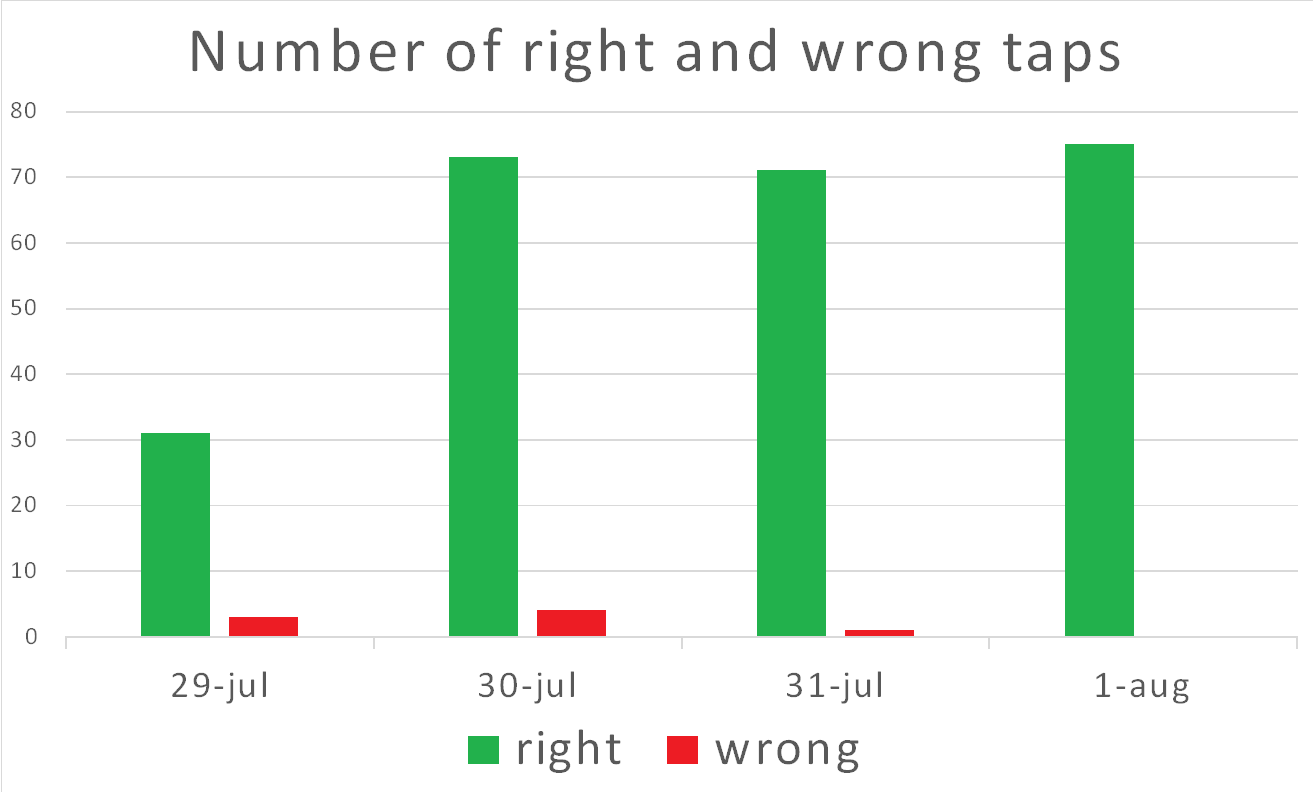
\includegraphics[width=2.6in]{usage_results/1_right_wrong.png} }}%
    \qquad
    \subfloat[User 2]{{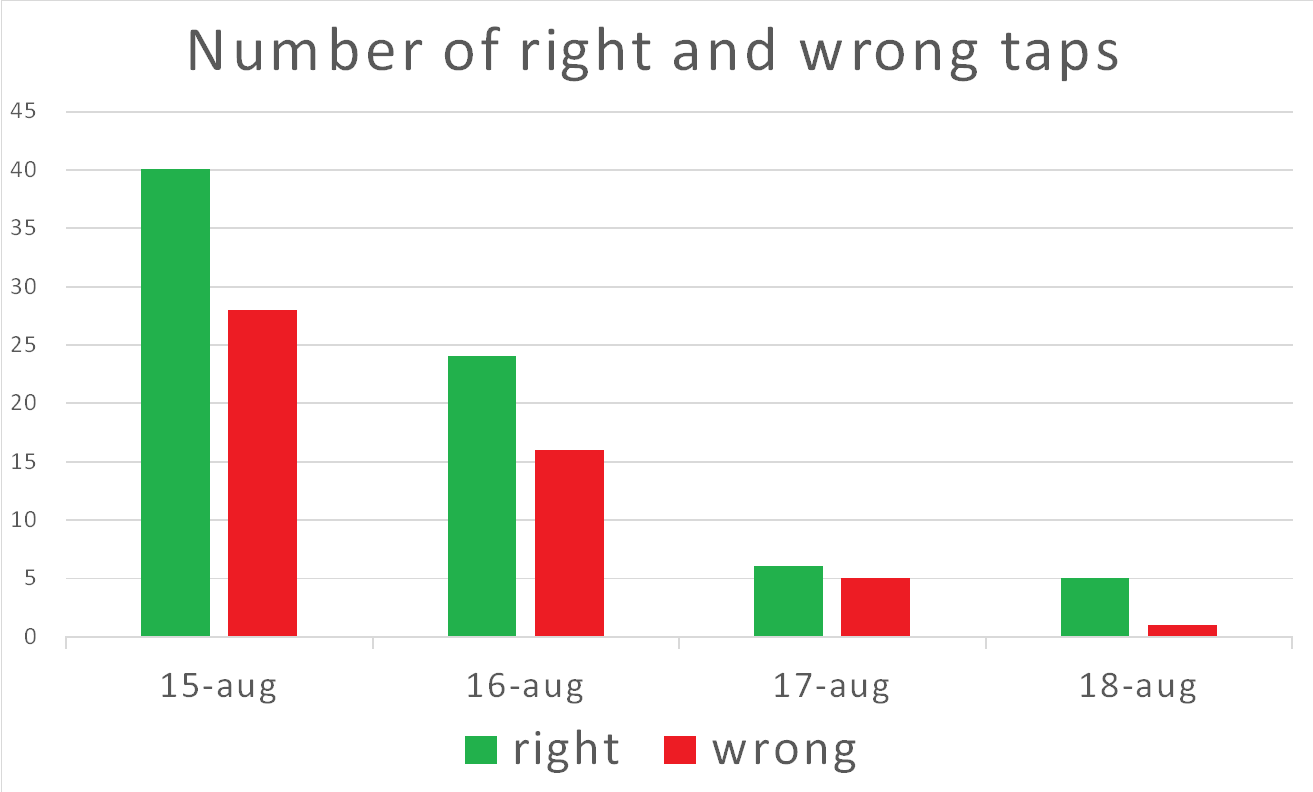
\includegraphics[width=2.6in]{usage_results/2_right_wrong.png} }}%
    \caption{Number of right and wrong clicks for users 1 and 2}%
    \label{fig:right wrong 1 2}%
\end{figure}

\begin{figure}[H]%
    \centering
    \subfloat[User 3]{{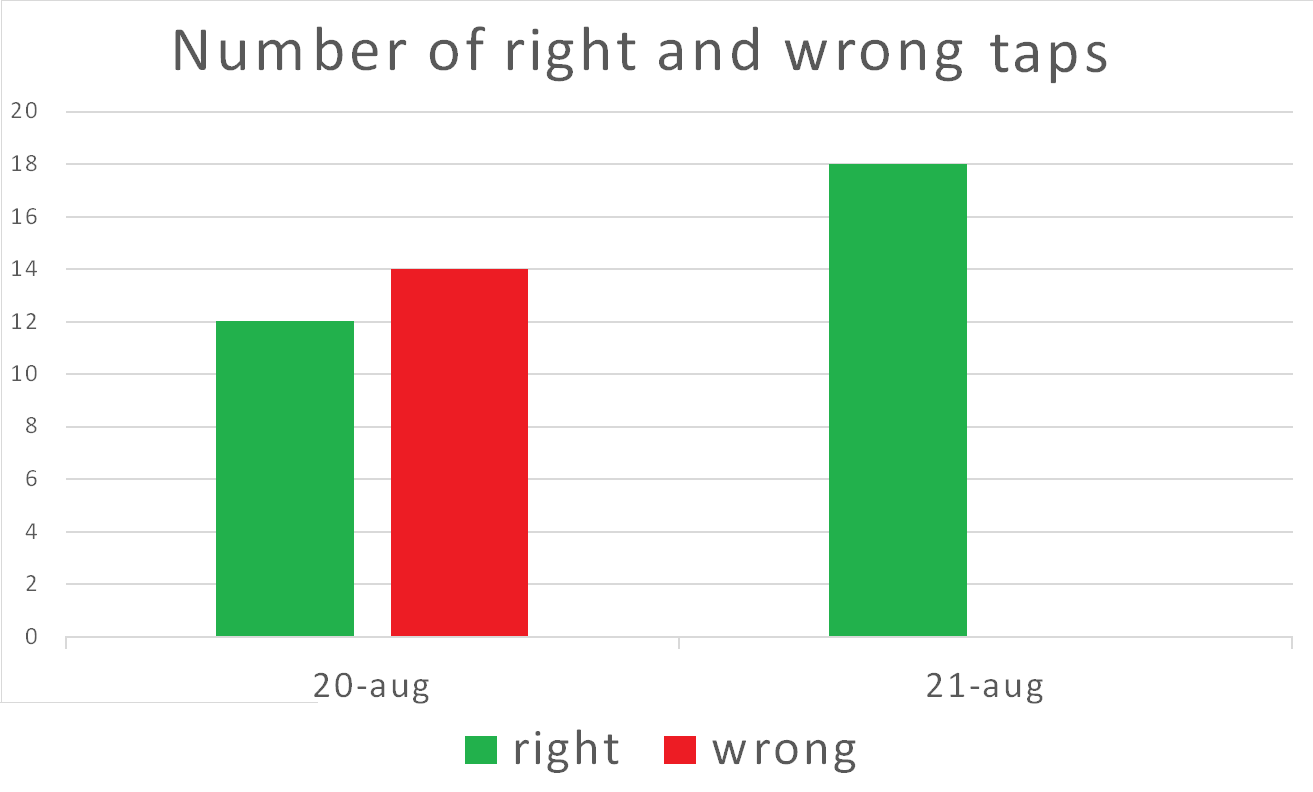
\includegraphics[width=2.6in]{usage_results/3_right_wrong.png} }}%
    \qquad
    \subfloat[User 4]{{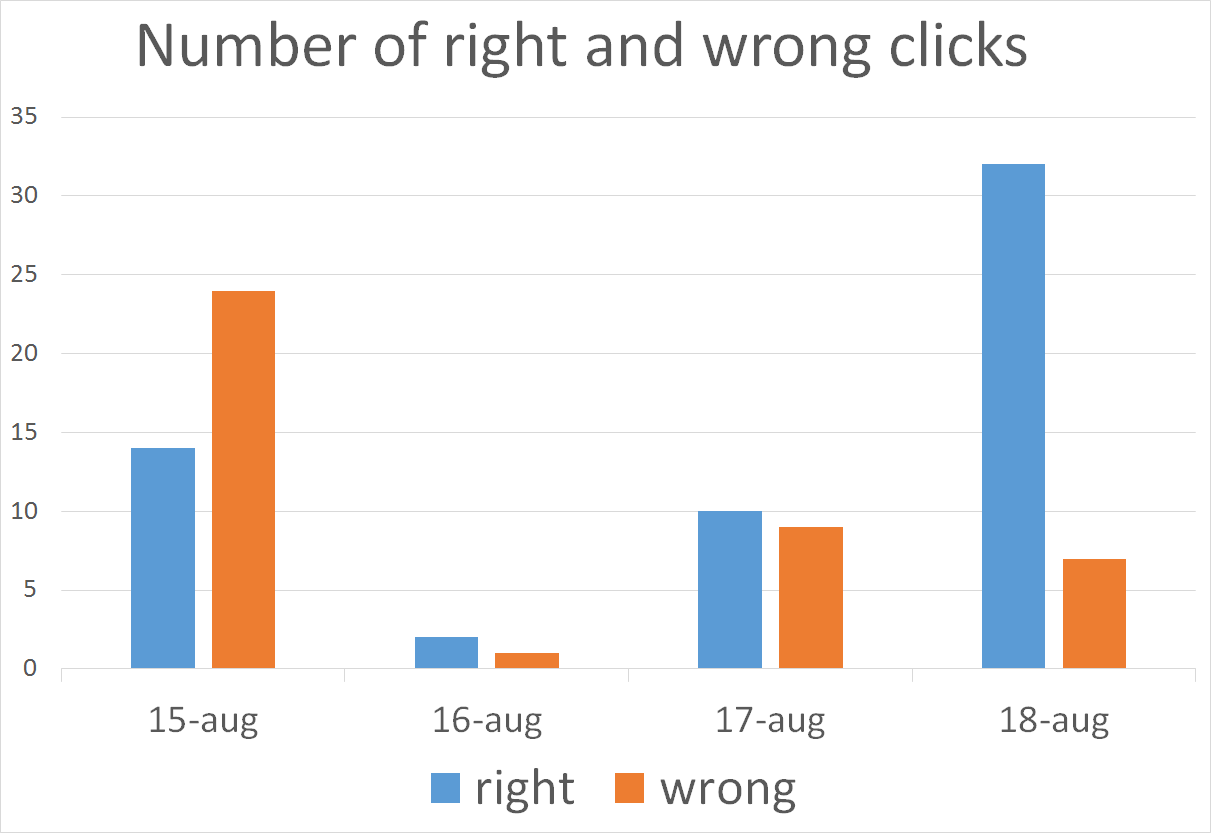
\includegraphics[width=2.6in]{usage_results/4_right_wrong.png} }}%
    \caption{Number of right and wrong clicks for users 3 and 4}%
    \label{fig:right wrong 3 4}%
\end{figure}

\begin{table}[H]
\centering
\caption{User 1 average reaction time and total usage time}
\label{table time 1}
\begin{tabular}{| l | l | l |} 
\hline
\textbf{Date} & \textbf{Average} & \textbf{Time} \\ \hline 
29-07-2016 & 00:00:02 & 00:08:39 \\ \hline
30-07-2016 & 00:00:13 & 00:13:10 \\ \hline
31-07-2016 & 00:00:01 & 00:45:43 \\ \hline
01-08-2016 & 00:00:36 & 00:37:07 \\ \hline
\hline
\textbf{Average} & 00:00:07 & 00:26:10 \\ \hline
\textbf{Total} & & 01:44:39 \\ \hline
\end{tabular}
\end{table}

\begin{table}[H]
\centering
\caption{User 2 average reaction time and total usage time}
\label{table time 2}
\begin{tabular}{| l | l | l |} 
\hline
\textbf{Date} & \textbf{Average} & \textbf{Time} \\ \hline 
15-08-2016 & 00:00:08 & 00:19:45 \\ \hline
16-08-2016 & 00:00:02 & 02:15:03 \\ \hline
17-08-2016 & 00:00:02 & 00:36:00 \\ \hline
18-08-2016 & 00:00:02 & 00:01:00 \\ \hline
\hline
\textbf{Average} & 00:00:05 & 00:47:57 \\ \hline
\textbf{Total} & & 02:35:48 \\ \hline
\end{tabular}
\end{table}

\begin{table}[H]
\centering
\caption{User 3 average reaction time and total usage time}
\label{table time 3}
\begin{tabular}{| l | l | l |} 
\hline
\textbf{Date} & \textbf{Average} & \textbf{Time} \\ \hline 
21-08-2016 & 00:04:20 & 00:18:21 \\ \hline
22-08-2016 & 00:00:04 & 00:02:23 \\ \hline
\hline
\textbf{Average} & 00:02:12 & 00:10:22 \\ \hline
\textbf{Total} & & 00:20:44 \\ \hline
\end{tabular}
\end{table}

\begin{table}[H]
\centering
\caption{User 4 average reaction time and total usage time}
\label{table time 4}
\begin{tabular}{| l | l | l |} 
\hline
\textbf{Date} & \textbf{Average} & \textbf{Time} \\ \hline 
16-08-2016 & 00:03:54 & 00:37:23 \\ \hline
17-08-2016 & 00:00:03 & 04:05:46 \\ \hline
18-08-2016 & 00:12:34 & 00:28:02 \\ \hline
19-08-2016 & 00:02:30 & 00:13:41 \\ \hline
\hline
\textbf{Average} & 00:04:45 & 01:21:13 \\ \hline
\textbf{Total} & & 05:24:52 \\ \hline
\end{tabular}
\end{table}

\lstinputlisting[label=script, language=JavaScript, caption=script to get different session lengths]{source_code/script_research.js}

\section{Evaluating usage results}
\subsection{General usage}
The graph about the overall usage of the smartwatch tells something about the behavior of the users related to a smartwatch. From the graphs it can be seen that most of the time (53\% till 66\%) the smartwatch is used less than three seconds. This can be related to checking the time which could mean that the ratio between checking the time and learning words is roughly 50 to 50. This is in a well agreement with the design where 50\% of the screen is used for the time and the other 50\% for learning words.\\
The graphs also shows that a session on the smartwatch rarely lasts for more than 60 seconds. Apparently the smartwatch is not suitable or convenient enough to be constantly used for a long period. If the smartwatch is used for a session that lasts a couple of minutes then this will not be longer than fifteen seconds in most cases.

\subsection{Learning sessions}
The graph about the learning sessions shows a different distribution when it comes to the duration of the sessions. When the smartwatch is used to learn words, the session last for 5 till 60 seconds most of the time where the interval of 15 till 60 seconds is often the largest. Sessions that are used for learning and that last for more than 60 seconds are still a small percentage of all the sessions. In the graph from testperson 3 the distribution is a little bit skewed, this is probably due to a lack of results. This user didn't use the watch as often as the other users.

\subsection{Right and wrong}
If we look at all the graphs, it is easily seen that right is more often pressed than wrong. This might come as a surprise, since learning new words should start with more wrong then right. In the graph of testperson 1 (see fig. \ref{fig:right wrong 1 2}) this is shown extreme, this user had a German background. This might be a possible explanation for the absurd high number of right clicks. In the graph of testperson 2 (see fig. \ref{fig:right wrong 1 2}), a decrease in usage is seen. At 17 Augustus the watch it's battery was depleted, so therefore usage was less. At 18 Augustus usage was less since it was not a full day of usage, the user handed in the watch at noon. In the graph of testperson 3 (see fig. \ref{fig:right wrong 3 4}) it can be seen that the watch is unfortunately only used for 2 days, there is however a clear learning curve which can only be observed in the graphs of testperson 1 and 4. 

\subsection{Reaction time reveal to right/wrong}
The average reaction time between a `reveal' and a `right' or `wrong' differs per user. The first two participants had nearly the same reaction time which is quite fast compared to the other participants. A fast reaction could mean that they are fast learners and they do not have to spend a lot of time to learn the translation. This thought is confirmed by the bar chart where the two participants with a high reaction time had pressed `right' more often than `wrong'. \\
The other two participants had a much longer reaction time in comparison with the first two reaction times. It could be that these users needed more time to learn a new word and therefore they required more time to learn the translation of a certain word. In the bar chart of the testperson 4 (see fig. \label{fig:right wrong 3 4}) it can be seen that in the first day `wrong' is pressed more than `right' what could indicate that the user was confronted with some hard-to-learn words. 

\section{Questionnaires results}
In order to get even more feedback from the user it was decided to let them answer a questionnaire after their test period. The purpose was to get specific information about the app which cannot be obtained by only using the events. Although the test group was really small, it only consisted of four persons, we can still learn from it. The questionnaire was divided into two sections, questions related to:
\begin{itemize} 
\item general information about the user (i.e., what kind of users do we have)
\item the usage of the smartwatch app.
\end{itemize}
In the sections below the results are summarized and evaluated, the questionnaire can be found in appendix \ref{questionnaire} and the answers of the users in appendix \ref{questionnaire answers}.

\subsection{General information about the user}
All four of the users were relatively young, the youngest person was 22 and the oldest 34. It can thus be concluded that the test group was quite young. This could mean that they prefer certain ways of learning which fits the generation. What also was interesting to see was that people don't invest much time in learning new words. This could simply mean that they don't have much time, or that they just hate learning new words for long periods of time. Either case using the smartwatch app helps them invest more time in learning new words using micro learning. For the people who already were learning, the most frequent method was by reading texts in the other language. This would suggest that using the Zeeguu ecosystem (as explained in related work) in combination with the smartwatch is way that people who are enthusiastic about learning a new language would like. 

\subsection{Smartwatch app usage}
In general the reactions to the design were positive, the context function might need a larger font, but this will also result in more words being removed from the list, since the context won't fit on the screen. There were also some complains about not being able to find all the features the app offers. This was due to not having instructed some of the testers properly, but also because some features might not be very logical to find. The settings for example could be find by double tapping the time. This may not be the most convenient place for the user. A solution would be to have a sort of short instruction manual in the app itself, or to make some small button on the screen for settings. There were two interesting features mentioned that people would like to have in app. The first one was a pronunciation function, this however is hard to implement, because the Samsung Gear S2 does not have a speaker built in. Another feature which was mentioned was ``I don't want to learn this word'', one way of doing this would be to combine ``wrong translation''  and ``I don't want to learn this word'' to ``trash'', in either way the word has to be removed. The disadvantage would be less specific user feedback. The users used the app exactly how we hoped they would, they used it mostly when they had to wait for something. This is exactly what micro learning is all about, the small wait moments will now be filled.

\chapter {Conclusion and Future Work}

\section{Conclusion}

There are still some improvements that should be implemented in the app eventually. During the test period the users were dealing with a few crashes that were probably caused by functions that require an internet connection.\\
After analyzing the questionnaire it was clear that the users did not find all features the app has to offer them. This was caused by the lack of a proper instruction and the navigation that appeared to be not very intuitive for some features.

In the questionnaire the users stated the time they spent on learning new words daily. When we compared these results with the time the users spent on the smartwatch for learning, we can conclude that they spent more time on learning with the watch than without the smartwatch. This could be caused by the ability to have short learning session that is doable for the users. The users could experience some trouble with concentrating on the words for a long time, since the learning sessions without a smartwatch are much longer than with the smartwatch. Because the use of micro learning in combination with the app the users were able to increase the time they spent on learning.

The design of the app was simple and neat according to the participants. Hence this design will probably be used in the future.

After analyzing the results of the user study the questions stated in the introduction can be answered.\\
\textbf{How do users use a smartwatch application to accelerate the memorization process of somebody who is learning the vocabulary of a second language?}\\
The users that use a smartwatch application to learn new words use micro learning in order to learn new words. These short learning session can take place whenever the user has some time left. A few examples mentioned in the questionnaire are waiting for the traffic lights, taking the elevator or during watching television. 

\begin{itemize}
\item \textbf{How long does a session on a smartwatch take (i.e., general usage)?}\\ 
Most of the sessions last for less than three seconds and sessions of more than 60 seconds hardly appear as can be seen in the results from the user study. The smartwatch is therefore not used for long sessions by our users. 
\item \textbf{How long does a learning session take on a smartwatch (i.e., only using \ttl app)?}\\
The duration of a learning session is between 5 and 60 seconds most of the time. From the four different intervals the group between 15 and 60 seconds was the largest. These short learning sessions are in alignment with micro learning.
\item \textbf{How long do users use the app daily on average?}\\
The time that the users spent daily on the app differs from one another. This difference between the daily usage of each user is too large to give a general answer to this question. The usage differs from one minute till four hours.
\end{itemize}


\section{Future work}
As far as we know this is the first time a smartwatch app was made for learning vocabulary. In this project we tried to give the user the best possible experience to make learning as efficient and fun as possible. Naturally there are still some interesting features that can be implemented to improve the functionality of the app. Some examples are:
\begin{itemize}
\item \textbf{Improvements on the server side}\\
Several events are sent to the server when the app is used. These events were used for the test results. However these events could also be used to personalize the learning process. Every user has a different learning curve that plots the time it takes before a word will be forgotten. It is therefore important that a learning app shows that word again, before the user forgets the translation. A recent research project developed at the RUG tried to calculate this curve in order to maximize the efficiency of a learning app\cite{slimstampen}.
The algorithm for the learning curve could be implemented on the server side where it could use the events to estimate the learning curve for all users. The algorithm will send a word to the watch that the user should learn according to his learning curve. The downside of this approach for the used smartwatch model will be that the watch should constantly be connected to the internet to keep the learning curve up-to-date. The connection is also important for receiving new words from the server. There are smartwatch models that support 3G and therefore keeping a connection with the internet should not be a problem for these models.
\item \textbf{Knowing the form of the word}\\
In the `Related Work' chapter some techniques are mentioned which could improve the time it takes to learn new words. One of these techniques was categorizing the words into different forms, like: verbs, nouns or prepositions etc. so it is clear for the learner in which situation the word should be used. We are still unsure whether there is a database with the form for different words. If it exists, the app could show this form for every word although it will be hard to find space on the small screen.
\item \textbf{Pronunciation of a word}\\
After the test period almost all the users would like to have a pronunciation function. The smartwatch model we used did not have speakers, so this function would not work for this model. However, there are models which do have speakers and there are databases available with the pronunciation of a lot of words in different languages which means that this idea could be implemented in a later version of the app. 
\item \textbf{Pronounce the word aloud}\\
Another way to improve learning is to say the translation aloud. It can be read in the `Related Work' chapter that pronouncing a word aloud helps the saving process in the brains. The smartwatch model we used has a build-in microphone like many more models. This makes it possible to check if the user says something. This function could even be improved by verifying if the word is pronounced the right way.
\item \textbf{Avoid interference with words of similar spelling or meaning}\\
Words with a similar spelling or meaning should not be shown one after another in order to prevent confusion. This would require an algorithm and a database that decides whether two words have a similar spelling and whether these words have a similar meaning.
\item \textbf{Improve functionality of the app}\\
The method for showing new words on the app can be improved by showing the word and the translation simultaneously if it is the first time the user sees that word. After the first time the word and the translation can be shown in the same manner the app is showing the words in the latest version.

Since knowing the context of a certain word is important for the learning process, the `reveal' button could be split in two buttons with on the left the option to show the context and right the option to reveal the translation. The user will then be able to make an educated guess when reading the context of the word. In the latest version this is not possible since the option `show context' is only available when the translation is already revealed.

The settings should be opened when the user taps the time and double tap on the time should change the background. Changing the background is less important than the settings and thus entering the settings should need less afford than changing the background.

\end{itemize}

\begin{appendices}
\chapter{Test Cases}
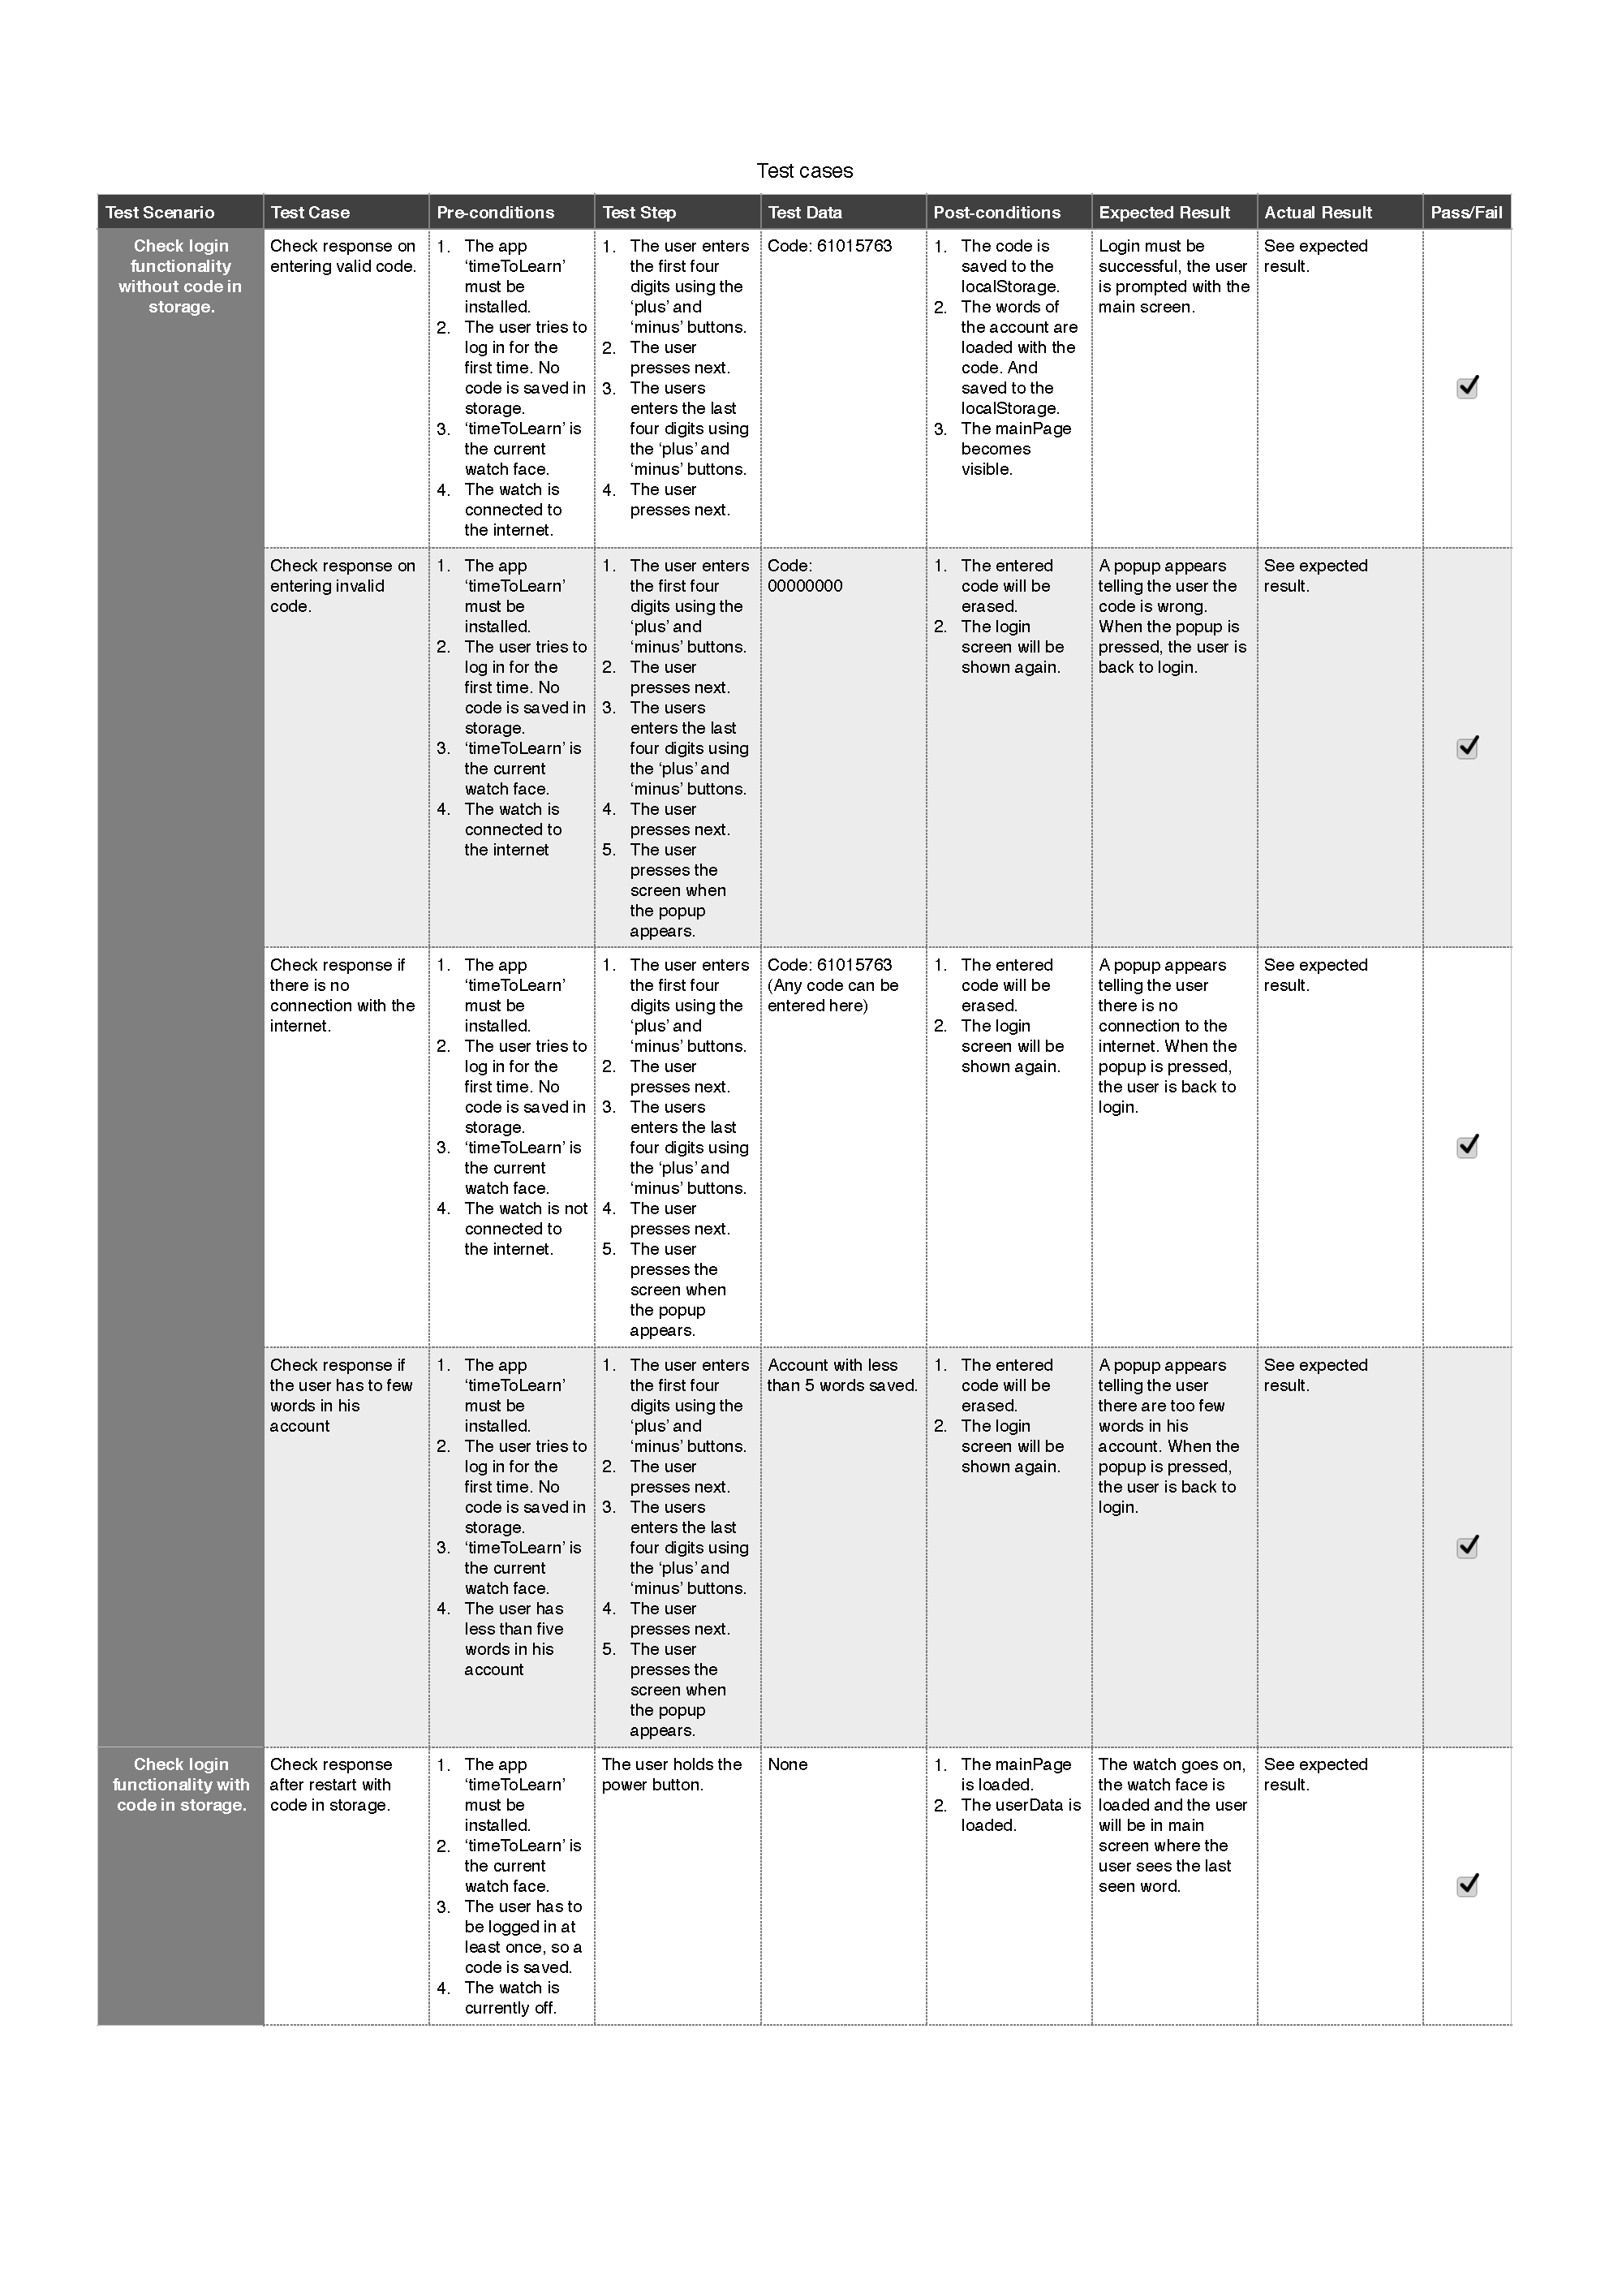
\includepdf[pages=-]{test_cases.pdf}
\chapter{Questionnaire}
\label{questionnaire}

The questionnaire asked the following questions to the participants:
\section{General information}
\begin{enumerate} 
\item What is your age?
\item How many times a day are you checking the time? 
\item If you are learning new words, how much time do you spend daily on learning?
\item What is your native language?
\item In which language have you learned the words on the app?
\item What is your current language level in this language that you are learning?
\begin{itemize}
\item A1 - Beginner. Can recognize and use simple phrases.
\item A2 - Elementary. Using simple words, can describe his or her surroundings and communicate immediate needs.
\item B1 - Intermediate. Can understand the main points of clear standard speech. Can narrate an event, an experience or a dream.
\item B2 - Upper Intermediate. Can speak in a clear, detailed way on a number of subjects; express an opinion on current affairs, giving the advantages and disadvantages of the various options.
\item C1 - Advanced. Can use the language effectively and fluently in a social, professional or academic context.
\item C2 - Master. Can express him or herself precisely in a spontaneous, fluent way, conveying finer shades of meaning precisely.
\end{itemize}
\item For how many years have you been studying this language?
\item How much time do/did you spend daily on learning before the app?
\item How much words do/did you learn daily?
\item In what way are you learning the language? (multiple choices)
\begin{itemize}
\item I'm not learning it yet, but I will.
\item Reading texts in the other language.
\item Using a textbook.
\item Talking/chatting with other people speaking the foreign language.
\item Apps for the smartphone.
\item Other:... 
\end{itemize}
\end{enumerate}

\section{Questions after using the smartwatch app}
\begin{enumerate}
\item What do you think about the design? (e.g., Were the buttons large enough, was the text readable etc.)
\item Was it clear how the app should be used? If not, why?
\item Some people did not use all of the features: show context, I learned it, wrong translation, reverse and profile. If you also didn't, could you let us know why?
\item What didn't you like about the app?
\item Which features did you miss that would have been useful?
\item Which features did you like? 
\item What did you think about the medals with the achievements in the app? 
\item When did you use the app the most? (e.g., waiting for the bus) 
\item When you didn't know a word, did you reveal the translation instantly or did you take time to think about the answer?
\item Did you sometimes press right when you actually didn't really know the word? If so, what was the reason? 
\item What score would you give the TimeToLearn app from 1 to 10?
\item Would you recommend the TimeToLearn app to your friends? 
\begin{itemize} 
\item Yes
\item No
\end{itemize}
\end{enumerate} 
\chapter{Questionnaire answers}
\label{questionnaire answers}
In this appendix the answers of the users are included, in the user study we used numbers to separate the users. The same numbers are used here to separate the user.

\section{General information}
\begin{enumerate} 
\item What is your age?
\begin{enumerate}[label=(\roman*)]
\item 24
\item 22
\item 26
\item 34
\end{enumerate}
\item How many times a day are you checking the time? 
\begin{enumerate}[label=(\roman*)]
\item It depends if I am waiting or not. Moreover, I do it subconsciously. I would say: About 10-15 times
\item 24 approximately
\item 7
\item 10
\end{enumerate}
\item If you are learning new words, how much time do you spend daily on learning?
\begin{enumerate}[label=(\roman*)]
\item Once a day, maybe 10 minutes
\item 1 hour
\item 10 min
\item not much...
\end{enumerate}
\item What is your native language?
\begin{enumerate}[label=(\roman*)]
\item Dutch
\item Dutch
\item Romanian
\item Romanian
\end{enumerate}
\item In which language have you learned the words on the app?
\begin{enumerate}[label=(\roman*)]
\item German
\item German
\item Danish
\item German
\end{enumerate}
\item What is your current language level in this language that you are learning?
\begin{enumerate}[label=(\roman*)]
\item C2
\item B1
\item A2
\item B1
\end{enumerate}
\item For how many years have you been studying this language?
\begin{enumerate}[label=(\roman*)]
\item The first time having it in school was 13 years ago
\item 6 (only at school)
\item 1
\item 3
\end{enumerate}
\item How much time do/did you spend daily on learning before the app?
\begin{enumerate}[label=(\roman*)]
\item None
\item none
\item Almost at all
\item not learning daily...
\end{enumerate}
\item How much words do/did you learn daily?
\begin{enumerate}[label=(\roman*)]
\item I picked about 5-6 words a day
\item none
\item Around 14
\item i didn't put time aside daily...
\end{enumerate}
\item In what way are you learning the language? (multiple choices)
\begin{enumerate}[label=(\roman*)]
\item 
\begin{itemize}
\item Reading texts in the other language 
\item Talking/chatting with other people speaking the foreign language.
\end{itemize}
\item I am not learning it yet, but I will.
\item 
\begin{itemize}
\item Reading texts in the other language
\item Using a textbook
\item Talking/chatting with other people speaking the foreign language.
\end{itemize}
\item Reading texts in the other language.
\end{enumerate}
\end{enumerate}

\section{Questions after using the smartwatch app}
\begin{enumerate}
\item What do you think about the design? (e.g., Were the buttons large enough, was the text readable etc.)
\begin{enumerate}[label=(\roman*)]
\item The design was great!
\item The design was alright, it was excellently readable.
\item The design was overall ok, it is simple and easy to use. You need to get closer to read the word in the sentence but that's an extra function.
\item context was not large enough i was missing an ``i don't want to learn this word" option. 
\end{enumerate}
\item Was it clear how the app should be used? If not, why?
\begin{enumerate}[label=(\roman*)]
\item It didn't come naturally to me that there were more options in the app, like ``I have learned the word". So I got the same words over and over, that I already knew.
\item It was clear from the instructions which I obtained from Niels, but to do it myself I think it would be confusing
\item Yes, it was quite clear. I was not sure when the words will be removed from the list and that's why I used the function 'I know the word, don't show it again'
\item clear for me
\end{enumerate}
\item Some people did not use all of the features: show context, I learned it, wrong translation, reverse and profile. If you also didn't, could you let us know why?
\begin{enumerate}[label=(\roman*)]
\item Because I didn't know the app had these features. A small tutorial might have done the job? Or a message ``You haven't used all features of this app. Did you know that... "
\item I only used these features once. I have no specific reason why I didn't use them, I forgot they existed sometimes and other times I just wanted a quick check if the translation I had in mind was correct.
\item I didn't use wrong translation because I was not sure about the translation, and didn't have time to check the word in another dictionary. It's still a very new language for me
\item reverse is not easy to find not always clear if a translation is wrong...
\end{enumerate}
\item What didn't you like about the app?
\begin{enumerate}[label=(\roman*)]
\item The translations weren't always correct in the context, as I sometimes already knew what it meant. It does have a option to choose a different translation, but a person learning a new language wouldn't know the exact word. That's just a problem with translation sites though and not the app itself. During testing the app screen froze like 2-3 times and sometimes reacted a bit slow.
\item None.
\item The fact that I was not sure if it is the right translation and also, that I couldn't hear the pronunciation
\item nothing
\end{enumerate}
\item Which features did you miss that would have been useful?
\begin{enumerate}[label=(\roman*)]
\item As explained earlier: A feature to encourage you to fully use the app or a small tutorial, as I was new to the app.
\item Maybe some feature to learn the pronunciation as well.
\item pronunciation
\item i would like to be able to see the context before the answer, maybe the context would help me remember the answer
\end{enumerate}
\item Which features did you like? 
\begin{enumerate}[label=(\roman*)]
\item Achievements and the general looks
\item The context feature is really helpful in my opinion although I didn't use it much.
\item The `show the word in the context' button
\item like being able to learn vocabulary in elevators
\end{enumerate}
\item What did you think about the medals with the achievements in the app? 
\begin{enumerate}[label=(\roman*)]
\item Great!
\item I did not pay much attention to this.
\item Were fun at the beginning but would not be so interesting on long term
\item Yes (I liked it)
\end{enumerate}
\item When did you use the app the most? (e.g., waiting for the bus)
\begin{enumerate}[label=(\roman*)]
\item Waiting, before going to sleep and out of boredom
\item When I was doing nothing at all or waiting, mostly in the evenings while watching tv and so on.
\item Waiting for the green light while biking
\item when waiting for people, or things (e.g. elevator)
\end{enumerate}
\item When you didn't know a word, did you reveal the translation instantly or did you take time to think about the answer?
\begin{enumerate}[label=(\roman*)]
\item Most of the time instantly. I was impatient and curious to know what it meant.
\item sometimes I accidentally hit reveal translation but mostly I tried to think about the correct translation.
\item Waited few seconds but not very long
\item i would reveal the answer if i didn't know the word
\end{enumerate}
\item Did you sometimes press right when you actually didn't really know the word? If so, what was the reason?
\begin{enumerate}[label=(\roman*)]
\item No, perhaps a miss click
\item Yes sometimes, only by accident.
\item Seldom, and if so, because I believe the word it's not so important
\item maybe... so i can feel good about myself
\end{enumerate}
\item What score would you give the TimeToLearn app from 1 to 10?
\begin{enumerate}[label=(\roman*)]
\item No, perhaps a miss click
\item 9
\item 7 (maybe develop it for smartphones, I don't like having a watch, would like to have also pronunciation and a very accurate translation)
\item 8/10
\end{enumerate}
\item Would you recommend the TimeToLearn app to your friends? 
\begin{enumerate}[label=(\roman*)]
\item Yes
\item Yes
\item Yes
\item Yes
\end{enumerate}
\end{enumerate} 


\end{appendices}


%END Doc
%-------------------------------------------------------

\bibliography{bibliography.bib}
\bibliographystyle{plain}

\end{document}